\documentclass[11pt,a4paper]{ctexart}
%以下为所使用的宏包
\usepackage{ulem}%下划线
\usepackage{amsmath,amsfonts,amssymb,amsthm,amsbsy}%数学符号
\usepackage{graphicx}%插入图片
\usepackage{booktabs}%三线表
%\usepackage{indentfirst}%首行缩进
\usepackage{tikz}%作图
\usepackage{appendix}%附录
\usepackage{array}%多行公式/数组
\usepackage{makecell}%表格缩并
\usepackage{siunitx}%SI单位--\SI{number}{unit}
\usepackage{mathrsfs}%数学字体
\usepackage{enumitem}%列表间距
\usepackage{multirow}%列表横向合并单元格
\usepackage[colorlinks,linkcolor=red,anchorcolor=blue,citecolor=green]{hyperref}%超链接引用
\usepackage{float}%图片、表格位置排版
\usepackage{pict2e,keyval,fp,diagbox}%带有斜线的表格
\usepackage{fancyvrb,listings}%设置代码插入环境
\usepackage{minted}%代码环境设置
\usepackage{fontspec}%字体设置
\usepackage{color,xcolor}%颜色设置
\usepackage{titlesec} %自定义标题格式
\usepackage{tabularx}%列表扩展
\usepackage{authblk}%titlepage作者信息
\usepackage{nicematrix}%更好的矩阵标定
\usepackage{fbox}%更多浮动体盒子



%以下是页边距设置
\usepackage[left=0.5in,right=0.5in,top=0.81in,bottom=0.8in]{geometry}

%以下是段行设置
\linespread{1.4}%行距
\setlength{\parskip}{0.1\baselineskip}%段距
\setlength{\parindent}{2em}%缩进


%其他设置
\numberwithin{equation}{section}%公式按照章节编号
\newenvironment{point}{\raggedright$\blacktriangleright$}{}
\newenvironment{algorithm}[1]{\vspace{12pt} \hrule\hrule \vspace{3pt} \noindent\textbf{\color[HTML]{E63F00}Algorithm } \,\textit{#1} \vspace{3pt} \hrule\vspace{6pt}}{\vspace{6pt}\hrule\hrule \vspace{12pt}} % 算法伪代码格式环境


%代码环境\lst设置
\definecolor{CodeBlue}{HTML}{268BD2}
\definecolor{CodeBlue2}{HTML}{0000CD}
\definecolor{CodeGreen}{HTML}{2AA1A2}
\definecolor{CodeRed}{HTML}{CB4B16}
\definecolor{CodeYellow}{HTML}{B58900}
\definecolor{CodePurPle}{HTML}{D33682}
\definecolor{CodeGreen2}{HTML}{859900}
\lstset{
    basicstyle=\tt,%字体设置
    numbers=left, %设置行号位置
    numberstyle=\tiny\color{black}, %设置行号大小
    keywordstyle=\color{black}, %设置关键字颜色
    stringstyle=\color{CodeRed}, %设置字符串颜色
    commentstyle=\color{CodeGreen}, %设置注释颜色
    frame=single, %设置边框格式
    escapeinside=`, %逃逸字符(1左面的键),用于显示中文
    %breaklines, %自动折行
    extendedchars=false, %解决代码跨页时,章节标题,页眉等汉字不显示的问题
    xleftmargin=2em,xrightmargin=2em, aboveskip=1em, %设置边距
    tabsize=4, %设置tab空格数
    showspaces=false, %不显示空格
    emph={TRUE,FALSE,NULL,NAN,NA,<-,},emphstyle=\color{CodeBlue2}, %其他高亮}
}


%节标题格式设置
% \titleformat{\section}[block]{\large\bfseries}{Exercise \arabic{section}}{1em}{}[]
% \titleformat{\subsection}[block]{}{    \arabic{section}.(\alph{subsection})}{1em}{}[]
% \titleformat{\subsubsection}[block]{\normalsize\bfseries}{    \arabic{subsection}-\alph{subsubsection}}{1em}{}[]
% \titleformat{\paragraph}[block]{\small\bfseries}{[\arabic{paragraph}]}{1em}{}[]


% \titleformat{\sectioncommand}[shape]{format}{title-label}{sep}{before-title}[after-title]



% 中文字号
% 初号42pt, 小初36pt, 一号26pt, 小一24pt, 二号22pt, 小二18pt, 三号16pt, 小三15pt, 四号14pt, 小四12pt, 五号10.5pt, 小五9pt




\begin{titlepage}
    \title{High Dimensional Data Analysis}
    \author{Tuorui Peng\footnote{TuoruiPeng2028@u.northwestern.edu}}
    \date{\today}
\end{titlepage}



\begin{document}
    

\tableofcontents



\section{Outline}

总体来说我感觉高维可算是经典的渐进统计的一个发展。在渐进统计中我们研究的是$n\to\infty$时的性质,最主要的就是各类的依概率收敛和a.s.收敛,或者最多到渐进正态性的问题。但是对于更复杂的一些情况,我们还是要回到何谓“$\infty$”这个东西本身:我们总是需要先认识有限的情况,再将之推广到无穷,所以在高维统计中,我们需要关心“从无穷撤回一些”,也就是$n$大但不完全大的情况,关心一些参考量(最典型如loss,或者说excess risk)随$n$增大的时候的变化趋势,从而了解一些统计模型的样本性质。渐进统计能够成立所依赖的trick是:对于性质足够好的“平均行为”(比如大数定律),其中总会有东西被随机性给平均掉/互相抵消掉,对于$n\to\infty$的情况,我们简单地发现细粒度的细节全部消失了,只留下我们经常关心的粗粒度性质;而在高维统计中,我们进一步关心“在多大程度上(as a function of $n$)”这些细节被冲洗掉,以控制尾概率(tail probability)的形式出现,例如:
\begin{align*}
    \mathbb{P}\left( \left\vert \, \cdot \, -\mathbb{E}\left[ \, \cdot \,  \right] \geq t  \right\vert  \right) \leq \text{decaying function of }t
\end{align*}

一个典型的例子就是高维回归,比如$p$与$n$同步增长的情况。在传统渐进统计框架中($p=\mathrm{const}$)是无法处理这种问题的,而应该先撤回到有限的$n$,通过包含$n$的理论,将$p$引入之后才能解决高维回归的统计性质问题。

所以对高维问题的理解大致有几步,就像把大象塞进冰箱一样:首先比如我们要研究一个复杂的对象,比如一串随机变量的最大值,一组数据的empirical loss,一个高维矩阵的norm(在某种意义上的,比如秩/operator norm/vector norm/trace);之后大致确定$ \mathbb{E}\left[ \, \cdot \,  \right]  $的bound(as a function of e.g. $ n,p $);然后控制$ \, \cdot \, -\mathbb{E}\left[ \, \cdot \,  \right]  $的concentration。虽然只有几步,但是过程中需要处理很多细节:研究的对象(函数)需要有怎么样的性质才足够好,能够产生有效的concentration(以及如何relax对函数性质的限制)?期望如何估计?(因为可能很难计算,没有解析表达式)




\textbf{参考书目:}

\begin{itemize}[topsep=2pt,itemsep=0pt]
    \item[MJW] \textit{High-Dimensional Statistics: A Non-Asymptotic Viewpoint} by Martin J. Wainwright
    \item[RV] \textit{High-Dimensional Probability: An Introduction with Applications in Data Science} by Roman Vershynin
    \item[RH] \textit{High-Dimensional Statistics Lecture Notes} by Philippe Rigollet and Jan-Christian Hütter
    \item[RvH] \textit{Probability in High Dimension - APC 550 Lecture Notes} by Ramon van Handel
    \item[YW] \textit{Information Theoretic Methods for High-Dimensional Statistics} by yihong Wu
\end{itemize}

       





    





\section{Concentration Inequalities}

Concentration指的是随机变量在“某个值”附近不会偏离太远,最典型的例子就是Markov不等式:与期望的偏差被方差控制。综合来说有很多concentration的方法,核心基本上就是“控制尾部”(tail behaviour),以及一些主旨相似的方法,比如控制矩(或矩母函数)。除了直接控制随机变量,我们还希望研究控制随机变量的函数,以及相关随机过程的行为。这里给出的基本都是在最general的情况下的bound,对于一些特殊的问题则常常可以通过更仔细地处理得到更好的bound。


\subsection{Sub-Gaussian}


对于随机变量的尾部控制一个典型的例子就是研究所谓的“亚高斯型”(sub-Gaussian)型随机变量,它有如下几个等价表述:$X$ is sub-Gaussian if and only if there exists some $K_i>0$ such that
\begin{enumerate}[topsep=2pt,itemsep=2pt]
    \item 控制尾部概率:
    \begin{align*}
        \mathbb{P}\left( \left\vert X - \mathbb{E}\left[ X \right] \right\vert \geq t \right)  \leq 2e^{- {\color{red}t^2}/K_1^2},\quad \forall t \geq 0
    \end{align*}
    \item 控制所有阶矩:
    \begin{align*}
        \left( \mathbb{E}\left[ \left\vert X - \mathbb{E}\left[ X \right]  \right\vert^p \right] \right)^{1/p} \leq K_2{\color{red}\sqrt{p}},\quad \forall p \geq 1 
    \end{align*}
    亚高斯随机变量的参数也由此处的最小的$K_2$给出。
    \begin{align*}
        \left\Vert X \right\Vert _{\psi_2} := \sup_{p\geq 1} \frac{1}{\sqrt{p}} \left( \mathbb{E}\left[ \left\vert X - \mathbb{E}\left[ X \right]  \right\vert^p \right] \right)^{1/p}
    \end{align*}
    \item 控制矩母函数:
    \begin{align*}
        \mathbb{E}\left[ e^{\lambda\left( X - \mathbb{E}\left[ X \right] \right)} \right] \leq e^{{\color{red}\lambda^2}K_3^2/2},\quad \forall \lambda \in \mathbb{R} 
    \end{align*}
\end{enumerate}

这样我们就有了一类“性质比较好的”随机变量,也就是尾部行为不会特别离谱,我们能够在均值附近解决问题。这样的随机变量在高维统计中有很多应用,最重要的是Hoeffding bound:对于亚高斯零均值的$X=(X_1,\ldots,X_n)$,我们有$ \forall a\in \mathbb{R}^n $:
\begin{align*}
     \mathbb{P}\left( \left\vert \left\langle a,X \right\rangle  \right\vert \geq t  \right) \leq 2 \exp\left( -\frac{t^2}{\left\Vert a \right\Vert _2^2 \max_i \left\Vert X_i \right\Vert _{\psi_2} }^2 \right)
\end{align*}
取$a = \dfrac{ 1 }{ n } \mathbf{1}$,就得到关于均值的Hoeffding bound。

类似的“好的”随机变量还有sub-exponential型,它的尾部行为稍差一些:
\begin{align*}
    \mathbb{P}\left( \left\vert X-\mathbb{E}\left[ X \right]  \right\vert  \right) \leq 2e^{-{\color{red}t}/K_1},\quad \forall t \geq 0 \\
    \left( \mathbb{E}\left[ \left\vert X - \mathbb{E}\left[ X \right]  \right\vert^p \right] \right)^{1/p} \leq K_2{\color{red}p},\quad \forall p \geq 1
\end{align*}
其亚指数参数为
\begin{align*}
    \left\Vert X \right\Vert _{\psi_1} := \sup_{p\geq 1} \frac{1}{p} \left( \mathbb{E}\left[ \left\vert X - \mathbb{E}\left[ X \right]  \right\vert^p \right] \right)^{1/p}
\end{align*}

由此可以直接得到亚指数型与亚高斯型的关系。对于亚高斯的$X$:
\begin{align*}
    \left\Vert X \right\Vert _{\psi_2} \leq \left\Vert X^2 \right\Vert _{\psi_1} \leq 2 \left\Vert X \right\Vert _{\psi_2}
\end{align*}
仔细地展开矩母函数很容易证。

\subsection{Hoeffding's Inequality}
从随机变量出发我们可以bound相应的随机过程以及随机变量的函数。重要例子是Hoefdding不等式。对于独立的$ \{X_i\sim \text{Sub-Gaussian}\}_{i=1}^n $我们有
\begin{align*}
    \mathbb{P}\left( \left\vert \sum_{i=1}^n( X_i - \mathbb{E}\left[X_i \right])  \right\vert \geq t \right) \leq  2\exp\left( -\frac{t^2}{\sum_{i=1}^n \left\Vert X_i \right\Vert _{\psi_2}^2} \right) 
\end{align*}


\subsection{McDiarmid's Inequality}
另一个常用的不等式是McDiarmid不等式,适用于逐坐标bounded的函数(bounded-difference function),是鞅差bound的推论。
\begin{align*}
    \left\vert f(x_1,\ldots,x_n) - f(x_1,\ldots,x_{i-1},\tilde{x}_i, x_{i+1},\ldots, x_n) \right\vert  \leq c_i
\end{align*}
,有
\begin{align*}
    \mathbb{P}\left( f(X_1,\ldots,X_n) - \mathbb{E}\left[ f(X_1,\ldots,X_n) \right] \geq t \right) \leq \exp\left[ -\dfrac{ 2 t^2}{\sum c_i^2}  \right]
\end{align*}


\subsection{Bounds for Lipschitz Functions}
一个更为实用/常用的情形是bound Lipschitz函数的行为。因为很多时候我们想要bound住的是类似norm的东西,这些东西很多时候都是Lipschitz函数。对于$ L $-Lipschitz函数$ f:\, \mathcal{X}^n\mapsto \mathbb{R} $和$ X\sim \mathrm{ Gaussian }(0,I)  $
\begin{align*}
    \mathbb{P}\left( \left\vert f(X)-\mathbb{E}\left[ f(X) \right]  \right\vert \geq t \right) \leq 2\exp\left( -\dfrac{ t^2 }{ 2nL^2 } \right)
\end{align*}
也即:高斯r.v.经过$ L $-Lipschitz函数后的行为类似于亚高斯$ \mathrm{subGau}(L^2) $。



\subsection{Maximal Inequality}
对于亚高斯变量一个非常好的用处是:既然其尾部行为比较好,那么一组亚高斯变量的$ \max $的尾部行为也会比较好,表现在我们可以bound$ \mathbb{E}\left[ \max_{i\leq n} X_i \right]  $。

对于$ X_1,\ldots,X_n \sim \mathrm{ subGau }(\sigma ^2)  $有
\begin{align*}
    \mathbb{E}\left[ \max_{i\leq n} X_i \right] =& \mathbb{E}\left[  \dfrac{ 1 }{ \lambda  } \log\max e^{\lambda X_i} \right] \\
    \leq & \dfrac{ 1 }{ \lambda  } \log \mathbb{E}\left[ \max e^{\lambda  X_i} \right] \\
    \leq & \dfrac{ 1 }{ \lambda  } \log  \mathbb{E}\left[ \sum_{i=1}^n e^{\lambda  X_i} \right] \\
    \leq & \dfrac{ 1 }{ \lambda  } \log n + \dfrac{ 1 }{ \lambda  } \dfrac{ \lambda ^2 \sigma ^2 }{ 2 }\\
    =& \dfrac{ 1 }{ \lambda  } \log n + \dfrac{ \lambda \sigma ^2 }{ 2 },\quad \forall \lambda > 0
\end{align*}
优化$ \lambda $得到
\begin{align*}
    \mathbb{E}\left[ \max_{i\leq n} X_i \right] \leq \sigma \sqrt{ 2\log n } 
\end{align*}

由于上面我们并没有施加任何独立性条件,所以我们可以创建一个$ X_1,\ldots,X_n,-X_1,\ldots,-X_n $来得到对$ \max \left\vert X_i \right\vert  $的bound
\begin{align*}
    \mathbb{E}\left[ \max_{i\leq n} \left\vert X_i \right\vert  \right] \leq \sigma \sqrt{ 2\log 2n } 
\end{align*}

尾部概率则是简单地通过union bound得到
\begin{align*}
    \mathbb{P}\left( \max_{i\leq n} X_i >t \right) =& \mathbb{P}\left( \bigcup X_i>t \right)\\
    \leq & \sum_{i=1}^n \mathbb{P}\left( X_i>t \right) = n\mathbb{P}\left( X_1>t \right)\\
    \leq & n\exp\left( -\dfrac{ t^2 }{ 2\sigma ^2 } \right) 
\end{align*}

{\color{red}\textbf{Idea}:} 对有限个subGau的maximal的bound是很实用的,因为对于某个我们想要研究的无限集,我们可以通过寻找其有限大代表元素集合(比如covering number)来将整个无限集上的maximal bound转化为有限集上的maximal bound。见\ref{sec:Rademacher}节的相关讨论。

% \begin{itemize}[topsep=2pt,itemsep=0pt]
%     \item 例子:bound$ \mathbb{E}\left[ \mathop{ \max  }\limits_{\theta \in \mathrm{ Ball }_2(1) } \theta 'X  \right]  $,其中$ \mathrm{ Ball }_2(1)  $是半径为1的$ \ell_2 $球。$ d $维球有covering number$ N(\varepsilon) \leq  (1+2/\varepsilon)^d \lesssim \varepsilon ^{-d}$,所以
%     \begin{align*}
%         \mathbb{E}\left[ \mathop{ \max  }\limits_{\theta \in \mathrm{ Ball }_2(1) } \theta 'X  \right] 
%     \end{align*}
    
    
% \end{itemize}

    




\subsection{Others}
\begin{itemize}[topsep=2pt,itemsep=0pt]
    \item Bernstein's Inequality: 稍微更小心地处理sub-exp的尾部即可。对于零均值$ X_i\sim \mathrm{ subexp }(\lambda )  $有
    \begin{align*}
        \mathbb{P}\left( \bar{X}>t \right) \vee \mathbb{P}\left( \bar{X}<-t \right) \leq \exp [-\dfrac{ n  }{ 2 } (\dfrac{ t^2 }{ \lambda ^2 } \wedge \dfrac{ t }{ \lambda } )]   
    \end{align*}
    反映了这样一件事:亚指数在近处的行为类似于高斯($ t^2 $),在远处的行为类似于指数($ t $)。
    \item 鞅差序列$ \{(D_k,\mathcal{F}_k)\}{_{k=1}^\infty} $的bound。如果$ D_k|\mathcal{F}_k $是亚指数的$ \mathrm{sujbexp}(\nu _k, \alpha _k) $,那么和会有bound
    \begin{align*}
        \sum_{k=1}^n D_k \sim \mathrm{subexp}( \sqrt{ \sum_{k=1}^n \nu _k^2 }, \max \alpha _k )
    \end{align*}
    
    
    
    
\end{itemize}

    
\section{Random Process and Complexity Control}

一个随机过程
\begin{align*}
    X(t),\quad t\in T 
\end{align*}
是一个由指标集$ T $ index的随机变量,其中$ T $可能是连续/离散,可以是多维度的,甚至有一些其它几何结构。在高维统计的场景中$ T $经常是模型假设类$ \mathcal{H} $(的参数化$ \Theta $),而$ X_i(t) $可以是$ X_i(t)=\hat{f}(x_i)-\mathbb{E}\left[ \hat{f}(x_i) \right]  $或是$ X_i(t)=\ell(h(x_i;\theta),y_i)-\mathbb{E}\left[ \ell(h(x_i;\theta),y_i) \right]  $等等。我们通常关心的对象也是形如
\begin{align*}
    \mathbb{E}\left[ \mathop{ \sup }\limits_{t\in T} \sum_{i=1}^N X_i(t)  \right]  ,\qquad \mathbb{E}\left[ \mathop{ \sup }\limits_{t\in T} \left\vert \sum_{i=1}^N X_i(t) \right\vert  \right]
\end{align*}
的东西(一族零均值随机过程的上界). 笼统来说这和指标集$ T $的“大小”和“形状”有关,我们有诸多手段来控制(upper or lower bound)这些东西。


\subsection{Complexity Control Via Metric Entropy}

\subsubsection{Rademacher Complexity and Symmetrization}\label{sec:Complexity}
Complexity是从随机过程的角度对一个集合的“大小”和“形状良好”的描述,关于其应用见\ref{sec:Rademacher}节。对于一列\textbf{零均值}随机过程$ [X_1(t),\ldots,X_N(t)]:= \vec{X}(t) $,我们定义其Rademacher复杂度为\footnote{也有一些相关概念,包括Gaussian complexity:
\begin{align*}
    \mathcal{G}(T):= \mathbb{E}\left[ \sup_{t\in T} \left\vert \sum_{i=1}^N \varepsilon_i X_i(t) \right\vert  \right],\quad \varepsilon_i\sim \mathcal{N}(0,1) 
\end{align*}
或者Gaussian width:
\begin{align*}
    w(T):= \mathbb{E}\left[ \sup_{t\in T}  \sum_{i=1}^N \varepsilon_i X_i(t)   \right],\quad \varepsilon_i\sim \mathcal{N}(0,1) 
\end{align*}
}
\begin{align*}
    \mathcal{R}(T)= \mathbb{E}\left[ \sup_{t \in T} \left\vert \dfrac{ 1 }{ n } \sum_{i=1}^n \varepsilon_i X_i(t) \right\vert  \right],\quad \varepsilon_i\sim \text{Rademacher}(\{\pm 1\})
\end{align*}

可以如此理解:$ \vec{X}(t)\mapsto \left\langle \varepsilon ,\vec{X}(t) \right\rangle  $相当于是做了一个对称化的操作,我的理解是这让我们可以利用上零均值的条件,得到下面的bound:
\begin{align*}
    \dfrac{ 1 }{ 2 }\mathbb{E}\left[ \sup \left\vert \left\langle \varepsilon ,\vec{X}(t) \right\rangle   \right\vert  \right]   \leq \mathbb{E}\left[ \sup \left\vert \sum _i X_i(t) \right\vert  \right] \leq 2\mathbb{E}\left[ \sup \left\vert \left\langle \varepsilon ,\vec{X}(t) \right\rangle   \right\vert  \right]
\end{align*}
证明思路和\ref{sec:Rademacher}中的类似,通过反复将对称话操作拿出拿进,制备$ \vec{X}_t $的copies来实现转换。\footnote{
    不带绝对值的width版本也是可证的:
    \begin{align*}
        \dfrac{ 1 }{ 2 } \mathbb{E}\left[ \sup \left\langle \varepsilon ,\vec{X}(t) \right\rangle  \right] \leq \mathbb{E}\left[ \sup \sum_{i} X_i(t) \right] \leq 2\mathbb{E}\left[ \sup \left\langle \varepsilon ,\vec{X}(t) \right\rangle  \right]  
    \end{align*}
}



\subsubsection{Covering Number}
{\color{blue}本subsection余下部分本来接在ULLN control后,所以使用的是$ (X_\theta ,\Theta ) $或$ X_h,\mathcal{H} $这套记号,基本上作$ \theta \mapsto t,\, \Theta \mapsto T $即可接续上文。}

复杂度笼统来说就是一个集合的“大小”。在高维问题中我们很多时候关心的是一个无限集合,这个时候没办法用$ \mathrm{card} $来处理问题,退而求其次得我们研究covering number和packing number。也就是将集合$ \mathcal{H} $近似到某个精确度$ \varepsilon  $来研究。

\begin{figure}[htbp]
    \centering
    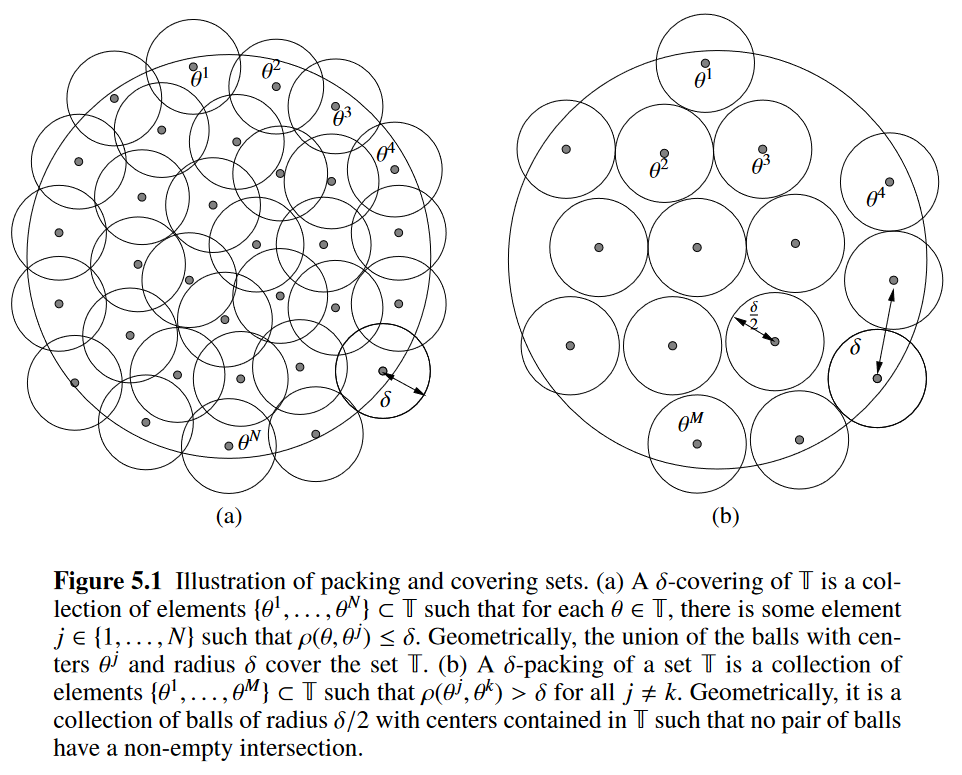
\includegraphics[width = 0.9\linewidth]{images/2024-08-05-14-29-34.png}
\end{figure}

\begin{itemize}[topsep=2pt,itemsep=2pt]
    \item Covering Number: 对于一个集合$ \mathcal{H} $,我们定义其$ \varepsilon $-covering number为
    \begin{align*}
        N(\varepsilon, \mathcal{H}, \Vert \cdot \Vert ) := \min\left\{ m\in \mathbb{N}:\, \exists h_1,\ldots,h_m\in \mathcal{H},\, \forall h\in \mathcal{H},\, \exists i\in [m],\, \Vert h-h_i \Vert \leq \varepsilon \right\}
    \end{align*}
    \item Packing Number: 对于一个集合$ \mathcal{H} $,我们定义其$ \varepsilon $-packing number为
    \begin{align*}
        M(\varepsilon, \mathcal{H}, \Vert \cdot \Vert ) := \max\left\{ m\in \mathbb{N}:\, \exists h_1,\ldots,h_m\in \mathcal{H},\, \forall i\neq j,\, \Vert h_i-h_j \Vert \geq \varepsilon \right\}
    \end{align*}

\end{itemize}

他们之间有如下很好的关系:
\begin{align*}
    M(2\varepsilon , \mathcal{H}, \Vert \cdot \Vert ) \mathop{ \leq  }\limits^{(i)}  N(\varepsilon, \mathcal{H}, \Vert \cdot \Vert ) \mathop{ \leq  }\limits^{(ii)} M(\varepsilon , \mathcal{H}, \Vert \cdot \Vert )
\end{align*}

\begin{proof}
    \begin{itemize}[topsep=2pt,itemsep=0pt]
        \item[$ (i) $] 考虑满足$ M(2\varepsilon, \mathcal{H}, \Vert \cdot \Vert ) $的$ \mathcal{M}(2\varepsilon, \mathcal{H}, \Vert \cdot \Vert ) \subset \mathcal{H} $及其中任意两个不同元素$ h_i,h_j $。取某个在$ \mathbb{B}_{\left\Vert \, \cdot \,  \right\Vert} (h_i, \varepsilon ) $中的点$ h $我们即有
        \begin{align*}
            \left\Vert h-h_j \right\Vert\geq \left\Vert h_i-h_j \right\Vert - \left\Vert h-h_i \right\Vert > 2\varepsilon - \varepsilon = \varepsilon ,\quad \forall h\in \mathbb{B}_{\left\Vert \, \cdot \,  \right\Vert} (h_i, \varepsilon ) 
        \end{align*}
        也就是说$ \mathcal{M}(2\varepsilon, \mathcal{H}, \Vert \cdot \Vert )\setminus \{h_i\} $不满足$ \varepsilon $-covering,又因为$ \varepsilon  $-covering是所有如此集合的$ \mathrm{card} $下界,所以$ N(\varepsilon, \mathcal{H}, \Vert \cdot \Vert ) \geq M(2\varepsilon, \mathcal{H}, \Vert \cdot \Vert ) $。

        \item[$ (ii) $] 考虑满足$ M(\varepsilon, \mathcal{H}, \Vert \cdot \Vert ) $的$ \mathcal{M}(\varepsilon, \mathcal{H}, \Vert \cdot \Vert ) \subset \mathcal{H} $。由于$ \mathcal{M}(\varepsilon, \mathcal{H}, \Vert \cdot \Vert ) $是满足$ \varepsilon  $-packing的最大集合,所以任意$ h\in\mathcal{H} $必满足
        \begin{align*}
            \exists h_i\in \mathcal{M}(\varepsilon, \mathcal{H}, \Vert \cdot \Vert ),\, \left\Vert h-h_i \right\Vert \leq \varepsilon 
        \end{align*}
        (也就是$ \varepsilon  $-covering)。因为如果不如此的话,$ M(\varepsilon, \mathcal{H}, \Vert \cdot \Vert )\cup \{h\} $就是一个更大的$ \varepsilon  $-packing,这与$ \mathcal{M}(\varepsilon, \mathcal{H}, \Vert \cdot \Vert ) $的最大性矛盾。所以$ N(\varepsilon, \mathcal{H}, \Vert \cdot \Vert ) \leq M(\varepsilon, \mathcal{H}, \Vert \cdot \Vert ) $。
        
        
    \end{itemize}
    
        
\end{proof}

所以我们只需能bound住其中之一即可控制集合的尺寸,一般是bound covering。

一个应用是通过这个方法控制某个集合的Gaussian复杂度,见Wainwright的书P. 136。核心方法是:对于零均值亚高斯过程$ \{X_\theta : \theta \in \Theta\} $(w.r.t metric $ \rho _X $),有如下的discretization bound
\begin{align*}
    \mathbb{E}\left[ \mathop{ \sup  }\limits_{\theta ,\tilde{\theta }\in \Theta} (X_\theta -X_{\tilde{\theta }})  \right]  \leq \underbrace{2\mathbb{E}\left[ \mathop{ \sup  }\limits_{\gamma ,\gamma '\in \Theta; \rho _X(\gamma ,\gamma ')\leq \varepsilon } (X_\gamma - X_{\gamma '} )  \right] }_\text{approximation error} + \underbrace{2\sqrt{ D^2\log N(\varepsilon , \Theta, \rho _X) } }_\text{estimation error},\quad \forall \varepsilon 
\end{align*}
其中$ D=\mathop{ \sup  }\limits_{\theta ,\tilde{\theta }\in \Theta} \rho _X(\theta ,\tilde{\theta })  $。亚高斯过程指的是
\begin{align*}
    \mathbb{E}\left[ e^{\lambda (X_\theta -X_{\tilde{\theta }} )} \right] \leq e^{\lambda^2 \rho _X(\theta ,\tilde{\theta} )^2/2} 
\end{align*}

上面的discretization bound的右边是一个$ \varepsilon  $的函数,我们再对$ \varepsilon  $优化就能trade-off两个error得到一个更好的bound。

以$ \mathcal{T}\subset \mathbb{R}^n $ with $ \ell_2 $ norm为例:
\begin{align*}
    \mathcal{G}(\mathcal{H})\leq \mathop{ \min  }\limits_{\varepsilon \in [0,D]}\Big\{ \varepsilon \sqrt{d} + 2\sqrt{ D^2\log N(\varepsilon , \mathcal{H}, \left\Vert \, \cdot \,  \right\Vert _2) }          \Big\}  
\end{align*}
具体例子见Wainwright的书P. 137。


\begin{proof}
    (Sketch)本质上大致是这么件事情:在$ \theta ,\tilde{\theta } $之间插入$ \gamma ,\gamma '\in \mathcal{N}(\varepsilon ,\Theta, \rho _X) $
    \begin{align*}
        \mathop{ \sup  }\limits_{\theta ,\tilde{\theta }\in \Theta} (X_\theta -X_{\tilde{\theta }}) \leq & \mathop{ \sup  }\limits_{\theta; \gamma \in \mathcal{N}(\varepsilon ,\Theta, \rho _X) } (X_\theta -X_{\gamma }) +{\color{red} \mathop{ \sup  }\limits_{\gamma ,\gamma '\in \mathcal{N}(\varepsilon ,\Theta, \rho _X) } (X_\gamma -X_{\gamma '})} + \mathop{ \sup  }\limits_{\tilde{\theta }; \gamma '\in \mathcal{N}(\varepsilon ,\Theta, \rho _X) } (X_{\gamma '} -X_{\tilde{\theta }}) \\
        \leq & 2 \mathop{ \sup  }\limits_{\gamma ,\gamma '\in \Theta; \rho _X(\gamma ,\gamma ')\leq \varepsilon } (X_\gamma - X_{\gamma '} ) +{\color{red} 2 \mathop{ \max  }\limits_{\theta _i \in \mathcal{N}(\varepsilon ,\Theta, \rho _X) } \left\vert X_{\theta _i}- X_{\theta _1} \right\vert } \\
        \leq& 2 \mathop{ \sup  }\limits_{\gamma ,\gamma '\in \Theta; \rho _X(\gamma ,\gamma ')\leq \varepsilon } (X_\gamma - X_{\gamma '} ) + 2\sqrt{ D^2\log N(\varepsilon , \Theta, \rho _X) }
    \end{align*}
\end{proof}




\subsubsection{Chaining}
上面的红色部分实际上是一个过于粗糙的近似,我们可以用chaining方法来改进,得到Dudley's entropy integral bound.
\begin{align*}
    \mathbb{E}\left[ \mathop{ \sup  }\limits_{\theta ,\tilde{\theta }\in \Theta} (X_\theta -X_{\tilde{\theta }})  \right]  \leq \underbrace{2\mathbb{E}\left[ \mathop{ \sup  }\limits_{\gamma ,\gamma '\in \Theta; \rho _X(\gamma ,\gamma ')\leq \varepsilon } (X_\gamma - X_{\gamma '} )  \right] }_\text{approximation error} + \underbrace{ 64\sqrt{2} \int_{\varepsilon /4}^{D/2} \sqrt{\log N(u, \Theta, \rho _X)} \,\mathrm{d}u   }_\text{estimation error},\quad \forall \varepsilon 
\end{align*}

\begin{proof}
    (Sketch)Chaining方法的主旨是,将$ \Theta $在$ \varepsilon _m = D\cdot 2^{-m} $精度下依次划分,然后对于每一个递进层$ \mathcal{N}(D2^{-m},\Theta, \rho _X)\leadsto \mathcal{N}(D2^{-(m+1)},\Theta, \rho _X) $,bound粗细粒度改进时approximation error:
    \begin{align*}
        \mathop{ \sup  }\limits_{\theta ,\tilde{\theta }\in \Theta} (X_\theta -X_{\tilde{\theta }}) \leq & \max_{\gamma ,\gamma '\in \mathcal{N}(D2^{-1},\Theta, \rho _X) } \vert X_\gamma - X_{\gamma '} \vert + \sum_{m=2}^{\sim \log_2 D} \max_{\beta \in \mathcal{N}(D2^{-m},\Theta, \rho _X) } \vert X_\beta  - X_{\text{sth in previous level}} \vert \\
        \leq & \sum_{m=1}^{\sim \log_2 D} 2D\cdot 2^{-m+1} \sqrt{\log N(D2^{-m}, \Theta, \rho _X) } \\
        \lessapprox & {\color{red}\mathrm{const} }\cdot \int^{D/2}_{\color{red} \varepsilon /4}\sqrt{\log N(u, \Theta, \rho _X) }\,\mathrm{d}u\tag{precise}\\
        \lesssim &C\cdot \int_{0}^{D/2} \sqrt{\log N(u, \Theta, \rho _X)} \,\mathrm{d}u\tag{rough}
    \end{align*}
    其中的红色部分是通过更精确的trivial计算可算出来的常数。
\end{proof}









\subsection{Sudakov-Fernique's Inequality for Gaussian Processes}
对于特别的$ X(t)\sim \mathcal{N}(0,\Sigma ) $有特殊的比较定理,Sudakov-Fernique's不等式。若$ (X(t))_{t\in T} $和$ (Y(t))_{t\in T} $是零均值\textbf{高斯}过程,有
\begin{align*}
    \left\Vert X_t-X_s  \right\Vert _2 \leq \left\Vert Y_t-Y_s  \right\Vert _2 ,\,\forall t,s\in T \Rightarrow \mathbb{E}\left[ \sup_t X_t \right] \leq \mathbb{E}\left[ \sup_t Y_t \right] 
\end{align*}

\textbf{Remark: }注意到这里的条件相当于在说$ \mathbb{E}\left[ X_tX_s \right] \geq \mathbb{E}\left[ Y_tY_s \right] $,这是一个“协方差的单调性”条件:内部“更不一致的”($ Y $)更容易有大的supremum。

\begin{proof}
    使用如下的引理:对于$ W\sim \mathcal{N}(0,\Xi) $和可导的$ h $,有
    \begin{align*}
        \mathbb{E}\left[ Wh(W) \right]   = \Sigma \mathbb{E}\left[ \nabla h(W) \right]  
    \end{align*}
    用密度函数做分部积分即可得到。

    然后对$ X(t),Y(t) $做插值:
    \begin{align*}
        Z_u(t)=\sqrt{u}X(t)+\sqrt{1-u}Y(t) 
    \end{align*}
    然后对合适的$ f $尝试证明$ \mathbb{E}\left[ f( Z_u(t) ) \right] $关于$ u $的单调性即可。具体来说取$ f(x)=\dfrac{ 1 }{ \beta  } \log \sum_i e^{\beta x_i}\mathop{ \to  }\limits_{\beta \to \infty} \max x_i  $即可。
    \begin{align*}
        \dfrac{\mathrm{d}^{}  }{\mathrm{d} u ^{} }\mathbb{E}\left[ f(Z(u)) \right]=&   \mathbb{E}\left[ \sum_{i=1}^n \dfrac{\mathrm{d}^{} f  }{\mathrm{d} \xi _i^{} } \left( \dfrac{ X(t) }{ 2\sqrt{u} } - \dfrac{ Y(t) }{ \sqrt{1-u} }   \right) \right] \\
        \mathop{ = }\limits^{\text{Lemma}}&  \dfrac{ 1 }{ 2\sqrt{u} } \sum_{i=1}^n \Sigma_X \cdot  \mathbb{E}\left[\sqrt{u} \nabla \dfrac{\mathrm{d}^{} f }{\mathrm{d} \xi _i^{} } \right] - \dfrac{ 1 }{ 2\sqrt{1-u} } \sum_{i=1}^n \Sigma_Y \cdot  \mathbb{E}\left[ \sqrt{1-u} \nabla \dfrac{\mathrm{d}^{} f }{\mathrm{d} \xi _i^{} } \right] \\
        =& \dfrac{ 1 }{ 2 } \sum_{i=1}^n\sum_{j=1}^n (\Sigma _{X,ij}-\Sigma _{Y,ij}) \mathbb{E}\left[ \dfrac{\mathrm{d}^{2} f }{\mathrm{d} \xi _i\xi _j^{} }\right] 
    \end{align*}
    trivially可以发现$ \dfrac{\mathrm{d}^{2} f }{\mathrm{d} \xi _i\xi _j^{} } \leq 0$,这样就能用单调性得到结论。
    
    
\end{proof}

\textbf{Application}: $ L $-Lipshitz函数的supermum bound。

\textbf{Example}: 对随机矩阵$ \{X_{ij} \mathop{ \sim  }\limits^{i.i.d.} \mathcal{N}(0,1) \}_{m\times n} $ 推bound $ \mathbb{E}\left[ |||X||| \right] \leq \sqrt{m}+\sqrt{n} $。

\textbf{Application}: 将$ \vec{X}(t) $设为我们想研究的过程,$ Y $是另一个相关的,容易研究的过程(or vice versa),通过Sudakov-Fernique's不等式我们可以得到$ \mathbb{E}\left[ \sup X(t) \right]  $的upper(或lower) bound。具体来说,
\begin{align*}
    (s,t)\mapsto \mathbb{E}\left[ (X(t)-X(s))^2 \right] ^{1/2}
\end{align*}
是$ \{X\} $空间中的正则度量(欧式度量),我们可以通过下面这个反向路径诱导出$ T $空间的(伪)度量:
\begin{figure}[H]
    \centering
    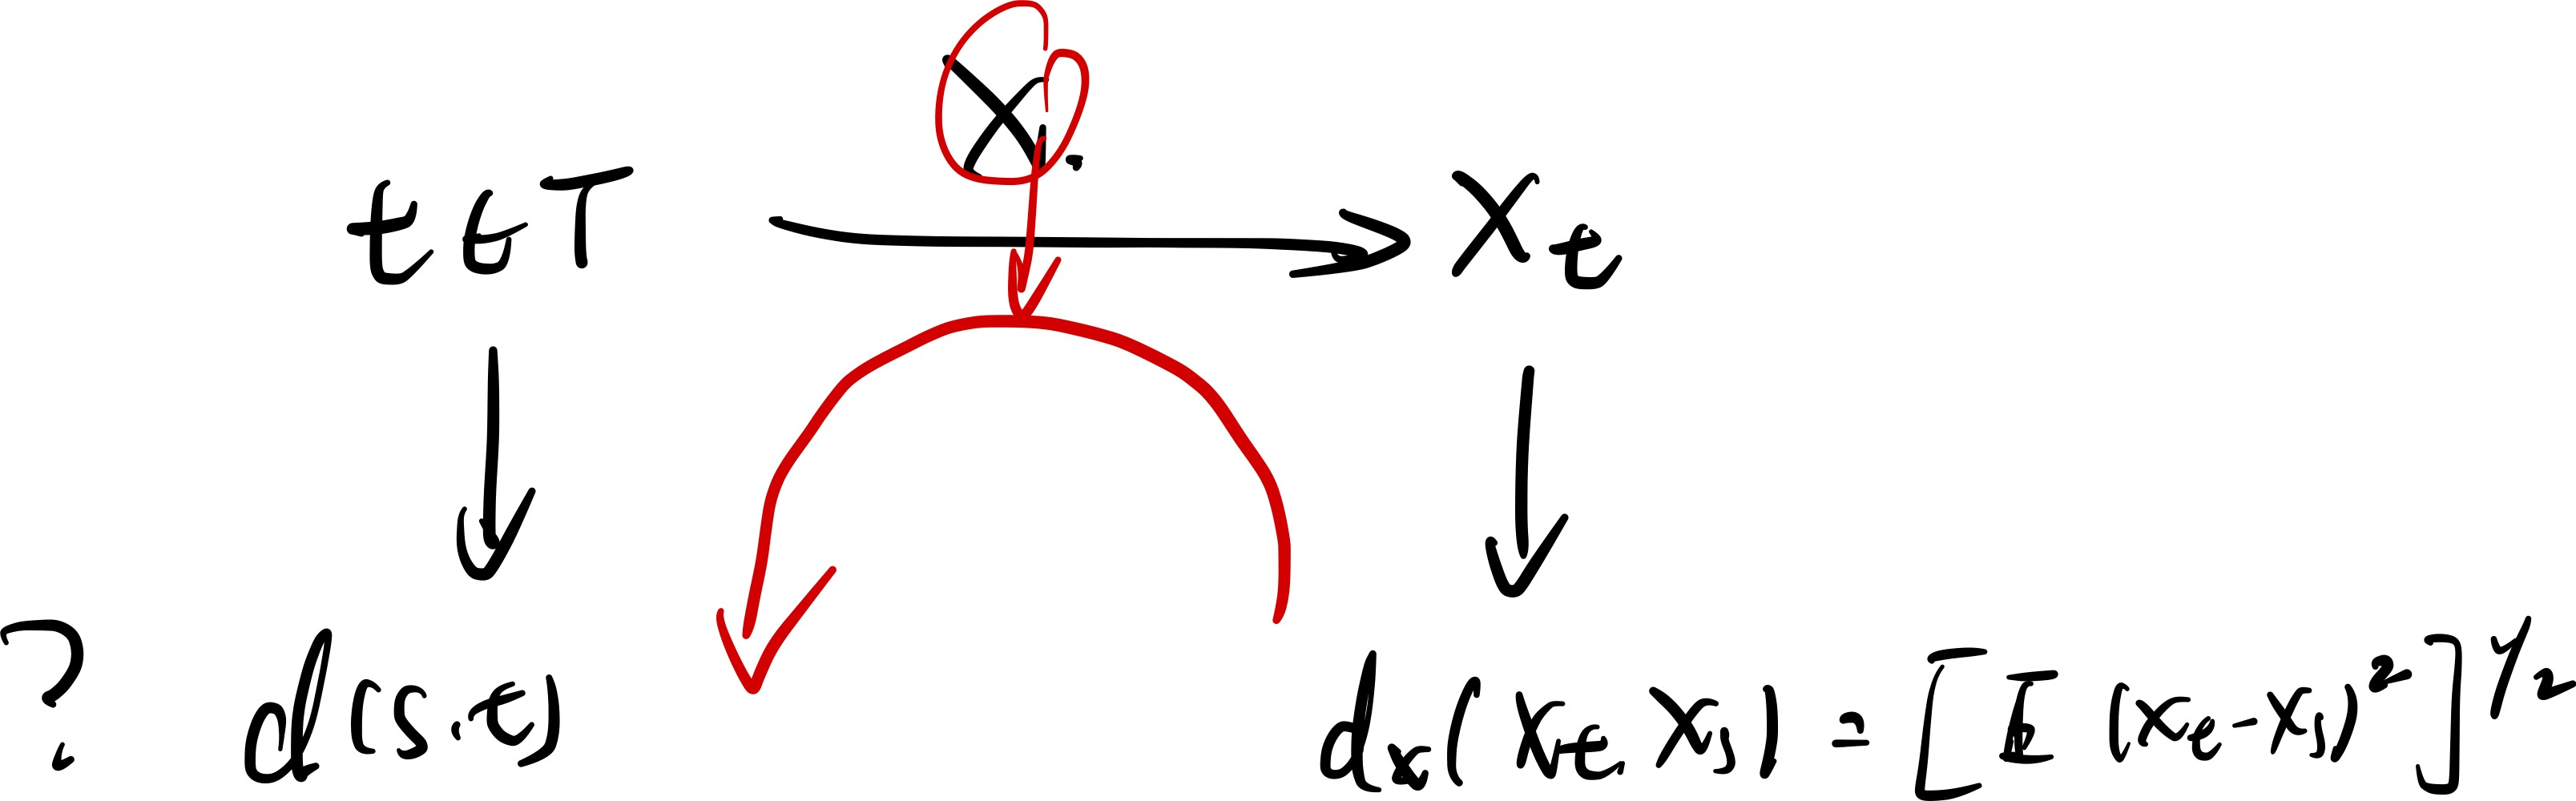
\includegraphics[width=0.7\linewidth]{images/2024-08-29-17-10-32.png}
\end{figure}
也就是$ X(\, \cdot \, )\mapsto d_T(\, \cdot \, ,\, \cdot \, ) $,这允许我们通过在$ X $欧式空间中研究$ T $的几何和尺寸(比如这里就可以应用Sudakov Ineq了)。

比如对于这样诱导出的$ T $空间的度量,我们可以进行$ T $的packing$ \mathcal{M}(\delta , T, d_T(\, \cdot \, ,\, \cdot \, ))= \mathcal{M}(\delta , X(T), \left\Vert  \right\Vert _2) $。进而通过$ Y_t=\text{ independent }N(0,\delta  ^2/2)  $即可得到一个$ X_t $的lower bound:
\begin{align*}
    \forall s,t\in\mathcal{M}(\delta , T, d_T(\, \cdot \, ,\, \cdot \, )):\, d^2(s,t)=\mathbb{E}\left[ (X_s-X_t)^2  \right]  \geq \varepsilon ^2  = \mathbb{E}\left[ N(0,\delta ^2)^2 \right]= \mathbb{E}\left[ (Y_t-Y_s)^2 \right]  
\end{align*}
故而得到(use MJW Exercise 2.11 or Vershynin Exercise 2.5.11)
\begin{align*}
    \mathbb{E}\left[ \sup X_t \right] \geq  \mathbb{E}\left[ \sup Y_i \right] \geq c\delta \sqrt{\log M(\delta , T, d_T(\, \cdot \, ,\, \cdot \, ))} 
\end{align*}


进一步由于有$ M(\delta ,T, \, \cdot \, )\geq N(\delta,T, \, \cdot \, ) $我们也可以将$ X_t $构造成一个容易的过程来bound覆盖数。

\textbf{Example:} 比如对于直径$ D\leq 1 $的$ N $顶点多边形$ P $
\begin{align*}
    \delta \sqrt{\log N(\delta ,T, \, \cdot \, )}\leq c \mathbb{E}\left[ \sup_{t\in P}\left\langle \varepsilon ,t \right\rangle  \right] = c\mathbb{E}\left[ \sup_{t\in \text{vertices}} \left\langle t,\varepsilon  \right\rangle  \right] \lesssim \delta \sqrt{\log N},\qquad \varepsilon \sim N(0,1)
\end{align*}
以此得到
\begin{align*}
    N(\delta ,T, \, \cdot \, )\lesssim N^{c/\varepsilon ^2} 
\end{align*}
(更精确的结果见Stat461-2023Fall exam Q2,得到$ C=1 $)




\subsection{本章小结}
我们有如下的bound:对于零均值高斯过程$ [X_1(t),\ldots,X_N(t)]:= \vec{X}(t) \, ,\, t\in T$,和$ \delta  $ covering number $ N(\delta ,T, \, \cdot \, ) $,有
\begin{align*}
    c\sup_{\delta >0}\delta \sqrt{\log N(\delta ,T, \, \cdot \, )} \mathop{ \leq  }\limits^{\text{Sudakov}} \mathbb{E}\left[ \mathop{ \sup  }\limits_{t\in T} X_t  \right] \mathop{ \leq  }\limits^{\text{Dudley}} C\int_0^{\mathrm{ Diam }(T)/2 } \sqrt{\log N(u,T, \, \cdot \, )} \,\mathrm{d}u
\end{align*}
其中更具体来说,Dudley side对于subGau也有效,上界$ \propto \left\Vert X_t  \right\Vert _{\psi_2} $.
















\section{Supervised Learning and Gereralization Bounds}

\subsection{Model and Empirical Risk}
机器学习中的典型框架是有监督学习(supervised learning),数据为$\mathcal{D}=\{(x_i,y_i)\}_{i=1}^n\subset \mathcal{X}\times \mathcal{Y}$,$X$与$Y$之间由函数$h:\, \mathcal{X}\mapsto \mathcal{Y}$刻画,我们即希望学习这样一个predictor(也就是我们的模型)。模型的好坏由一个损失函数(loss function)$\ell:\, \mathcal{Y}\times \mathcal{Y}\mapsto \mathbb{R}$来刻画,以反映估计值和真实值之间的差距。
\begin{itemize}[topsep=2pt,itemsep=0pt]
    \item Expected Loss (of a model $h$):
    \begin{align*}
        L(h) = \mathop{ \mathbb{E} }\limits_{X,Y} \left[ \ell\left( h(X),Y \right) \right] 
    \end{align*}
    \item Excess Risk:
    \begin{align*}
        E(h) = L(h) - \inf_{h'\in \mathcal{H}} L(h') 
    \end{align*}
    其中$\mathcal{H}$是我们的假设空间/假设类(hypothesis class)。我们的任务就是在$\mathcal{H}$中找到一个$h$,使得$E(h)$尽可能小,即取得最小的excess risk(对应泛化误差)。进一步,表达式后半部分的minimizer即为ground truth的$h^*$
    \begin{align*}
        h^*=\mathop{ \arg\inf  }\limits_{h'\in \mathcal{H}} L(h') 
    \end{align*}
     为了强调这一点我们overload$E$为$E(h,h^*)$。

    \item Emperical Loss:实际上我们并不能求出Expected Loss,只能用数据来近似之。
    \begin{align*}
        \hat{L}_n=& \hat{L}(\mathcal{D}_n)=\frac{1}{n} \sum_{i=1}^n \ell\left( h(x_i),y_i \right)
    \end{align*}
    已经提到,我们的目标是找到一个$h$,使得$E(h,h^*)$(或等价地,使$L(h)$)尽可能小,我们的估计量则自然是通过最小化$\hat{L}_n$来实现的,此估计量为$\hat{h}_n$。
    \begin{align*}
        \hat{h}_n=\mathop{ \arg\inf  }\limits_{h'\in \mathcal{H}} \hat{L}_n(h') 
    \end{align*}
    
    \item 参数化:对于假设类$\mathcal{H}$,很多情况下我们可以将其参数化到有限维空间上(比如线性模型$ \{ x\mapsto \beta \cdot x,\, \beta\in \mathbb{R} \} $,CDF经验估计$ \{x\mapsto \mathbf{1}_{(-\infty, t]}(x),\,t\in \mathbb{R}\} $),此时我们直接overload上述的$L$和$E$,用函数$h\in\mathcal{H}$的参数化$\theta \in \Theta$来表示$h$,即$L(\theta)$和$E(\theta, \theta ^*)$。(非参数化情形暂不讨论)
    \begin{align*}
    L(\theta )=& \mathop{ \mathbb{E} }\limits_{X,Y} \left[ \ell\left( h(X;\theta),Y \right) \right] \\ 
    E(\theta ,\theta ^*)=& L(\theta ) - \inf_{\theta' \in \Theta} L(\theta')= L(\theta ) - L(\theta ^*)\\
    \hat{L}_n(\theta )=& \frac{1}{n} \sum_{i=1}^n \ell\left( h(x_i;\theta),y_i \right)
    \end{align*}

\end{itemize}

一个好的模型应该能使得emperical risk $ E(\hat{\theta},\theta ^*) $尽可能小。在高维统计中我们关心:\textbf{随着样本量$n$的增大,$ E(\hat{\theta},\theta ^* ) $以何种趋势减小},即我们关心的是$E(\hat{\theta},\theta ^* )$的性质,它可以作如下分解:
\begin{align*}
    E(\hat{\theta},\theta ^* )=&\underbrace{L(\hat{\theta}) - \hat{L}( \hat{\theta} )}_{\text{I}} +  \underbrace{\hat{L}( \hat{\theta} ) - \hat{L}( \theta ^* )}_{\text{II}} + \underbrace{\hat{L}(\theta ^*) - L(\theta ^*)}_{\text{III}} 
\end{align*}
其中:
\begin{itemize}[topsep=2pt,itemsep=0pt]
    \item $ \text{II} $ 非正
    \item $ \text{III} $ 由于$ \theta ^* $是不带随机性的参数,并注意到$ \mathbb{E}_{\mathcal{D}\sim \theta ^*}\left[ \hat{L}(\theta ^*) \right]  = L(\theta ^*) $,这一项可以用经典的对均值的bound来控制,比如Hoeffding bound。
    \item[$ \mathbf{\Delta} $] $ \text{I} $比较麻烦,因为$ \hat{L} $是与样本有关的(有随机性)
    \begin{align*}
        \text{I}=& \mathbb{E}\left[ \ell ( h(X;\hat{\theta }), Y ) \right]  - \dfrac{ 1 }{ n  } \sum_{i=1}^n \ell ( h(x_i;\hat{\theta }), y_i ) 
    \end{align*}
    这需要\textbf{ULLN}(uniform law of large numbers)来控制
    \begin{align*}
         \text{I}\leq \sup_{\theta \in \Theta} \left\vert  \dfrac{ 1 }{ n  } \sum_{i=1}^n \ell ( h(x_i;\theta ), y_i ) - \mathbb{E}\left[ \ell ( h(X;\theta ), Y ) \right]  \right\vert := \left\Vert \mathbb{P}_n-\mathbb{P} \right\Vert _{\mathcal{H}(\Theta)} 
    \end{align*}
\end{itemize}
\begin{figure}[H]
    \centering
    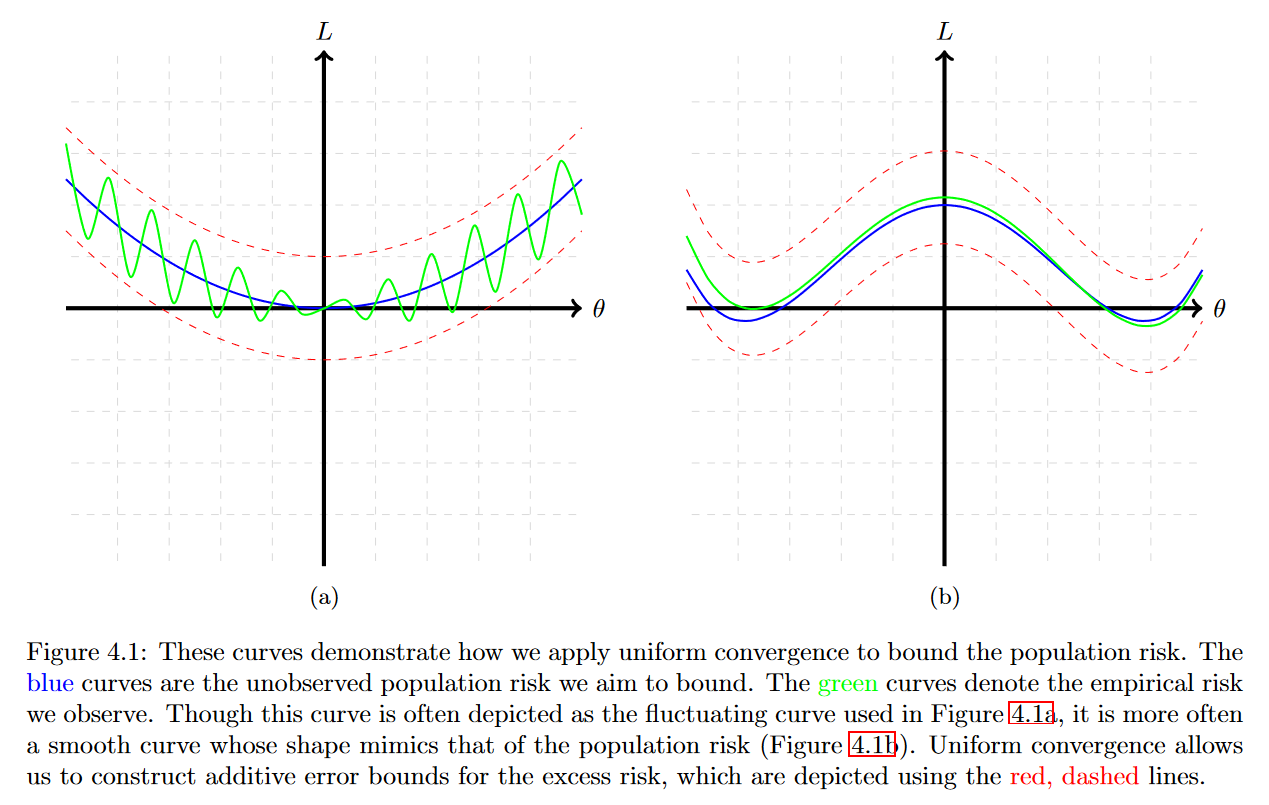
\includegraphics[width=\linewidth]{images/2024-07-30-20-09-08.png}
\end{figure}






\subsection{ULLN Control}

(To be modified)

\subsection{Via Rademacher Complexity}\label{sec:Rademacher}

控制$ \left\Vert \mathbb{P}_n-\mathbb{P} \right\Vert _{\mathcal{H}(\Theta)}  $的一种方法是用Rademacher复杂度(Rademacher complexity)

定义:对于一个集合$\mathcal{I}\equiv \{\imath \}\subset \mathbb{R}^n$,我们定义其Rademacher复杂度$ \mathcal{R}(\mathcal{I}) $为
\begin{align*}
    \mathcal{R}(\mathcal{I}) := \mathbb{E}\left[ \sup_{\imath \in \mathcal{I}} \left\vert \dfrac{ 1 }{ n } \sum_{i=1}^n \varepsilon_i \imath_i \right\vert  \right],\quad \varepsilon_i\sim \text{Rademacher}(\{\pm 1\})
\end{align*}
直观来说,如果集合$ \mathcal{I} $“很大”,那么我们就容易地总能找到$ \imath\in \mathcal{I} $很大,使得$ \left\langle \varepsilon ,\imath \right\rangle  $很大。更多关于Complexity的讨论见\ref{sec:Complexity}节。

我们会看到,risk就可以通过Rademacher复杂度来控制。这里的loss来自前面$ \mathrm{I} $部分,即我们希望控制
\begin{align*}
    \text{I}\leq \sup_{\theta \in \Theta} \left\vert  \dfrac{ 1 }{ n  } \sum_{i=1}^n \ell ( h(x_i;\theta ), y_i ) - \mathbb{E}\left[ \ell ( h(X;\theta ), Y ) \right]  \right\vert := \left\Vert \mathbb{P}_n-\mathbb{P} \right\Vert _{\mathcal{H}(\Theta)} 
\end{align*}
对于任意给定的数据$ \mathcal{D} $和假设空间$ \mathcal{H} $都会生成一个集合,为了克服掉数据的随机性我们再套一个期望,进一步定义这个场景下的Rademacher复杂度为
\begin{align*}
    \mathcal{R}(\mathcal{H}):= \mathbb{E}_{\mathcal{D}\sim \mathbb{P}}\left[ \mathcal{R}(\{\ell(h(x_i),y_i)\}_{h\in\mathcal{H}}) \right]  = \mathbb{E}_{\mathcal{D}\sim \mathbb{P}}\left[ \mathbb{E}_{\varepsilon\sim \mathrm{ Unif }\{\pm 1\} }\left[ \sup_{h\in\mathcal{H}} \left\vert  \dfrac{ 1 }{ n }\sum_{i=1}^n \varepsilon_i \ell(h(x_i),y_i) \right\vert  \right]  \right]
\end{align*}

这个情形下可以用Rademacher复杂度来控制risk的收敛性。定理如下:
    \begin{align*}
        \dfrac{ 1 }{ 2 } \mathcal{R}(\mathcal{H}) - \dfrac{ \mathop{ \sup  }\limits_{h\in\mathcal{H}}\mathbb{E}\left[ \left\vert\ell(h(x),y) \right\vert  \right] }{ 2\sqrt{n} }  \leq \mathbb{E}\left[ \left\Vert \mathbb{P}_n-\mathbb{P} \right\Vert_{\mathcal{H}}  \right]  \leq 2 \mathcal{R}(\mathcal{H})
    \end{align*}
    定理的证明用了一个神乎其技的对称话trick
\begin{itemize}[topsep=2pt,itemsep=0pt]
    \item[上界]: 
        


    \begin{proof}
        我们制备一个$ \mathcal{D}=\{(x_i,y_i)\}_{i=1}^n $的i.i.d. copy$ \tilde{\mathcal{D}}=\{(\tilde{x}_i,\tilde{y}_i)\}_{i=1}^n $. 于是可以在一些地方把$ \mathcal{D} $和$ \tilde{\mathcal{D}} $混合/替换,然后再用对称属性将混合的$ X $-$ Y $换成$ \varepsilon X $从而由risk gap过渡到complexity,实在是非常巧妙:
        \begin{align*}
            \mathbb{E}\left[ \left\Vert \mathbb{P}_n-\mathbb{P} \right\Vert _\mathcal{H} \right]= &\dfrac{ 1 }{ n }  \mathbb{E}_{\mathcal{D}}\left[ \mathop{ \sup  }\limits_{h\in\mathcal{H}}  \left\vert  \sum_{i=1}^n \ell\bigl(h(x_i), y_i\bigr) - \mathbb{E}_{\tilde{\mathcal{D}}}\left[ \ell\bigl(h(\tilde{x_i}, \tilde{y}_i)\bigr) \right]  \right\vert \right]   \\
            =& \dfrac{ 1 }{ n }  \mathbb{E}_{\mathcal{D}}\left[ \mathop{ \sup  }\limits_{h\in\mathcal{H}}  \left\vert \mathbb{E}_{\tilde{\mathcal{D}}} \sum_{i=1}^n \ell\bigl(h(x_i), y_i\bigr) - \ell\bigl(h(\tilde{x_i}, \tilde{y}_i)\bigr)  \right\vert \right] \\
            \mathop{ \leq  }\limits^{\text{Jensen}} & \dfrac{ 1 }{ n }  \mathbb{E}_{\mathcal{D},\tilde{\mathcal{D}}}\left[ \mathop{ \sup  }\limits_{h\in\mathcal{H}}  \left\vert  \sum_{i=1}^n \ell\bigl(h(x_i), y_i\bigr) - \ell\bigl(h(\tilde{x_i}, \tilde{y}_i)\bigr)  \right\vert \right]\\
            \mathop{ = }\limits^{\text{symmetrize}} & \dfrac{ 1 }{ n }  \mathbb{E}_{\mathcal{D},\tilde{\mathcal{D}}, \varepsilon }\left[ \mathop{ \sup  }\limits_{h\in\mathcal{H}}  \left\vert  \sum_{i=1}^n \varepsilon _i \big[ \ell\bigl(h(x_i), y_i\bigr) - \ell\bigl(h(\tilde{x_i}, \tilde{y}_i)\bigr) \big] \right\vert \right]\\
            \leq & 2 \mathbb{E}_{\mathcal{D},\varepsilon }\left[ \mathop{ \sup  }\limits_{h\in\mathcal{H}}  \left\vert  \sum_{i=1}^n \varepsilon _i \ell\bigl(h(x_i), y_i\bigr) \right\vert \right] \\
            =& 2 \mathcal{R}(\mathcal{H})
        \end{align*}
        
        
    \end{proof}

    \item[下界]: 
    \begin{proof}
        再用一次对称化得到另一边的bound

        \begin{align*}
            \mathbb{E}\left[ \left\Vert \mathbb{P}_n-\mathbb{P} \right\Vert _\mathcal{H} \right]= &\dfrac{ 1 }{ n }  \mathbb{E}_{\mathcal{D}}\left[ \mathop{ \sup  }\limits_{h\in\mathcal{H}}  \left\vert  \sum_{i=1}^n \ell\bigl(h(x_i), y_i\bigr) - \mathbb{E}_{\mathcal{D}}\left[ \ell\bigl(h({x_i}, {y}_i)\bigr) \right]  \right\vert \right]   \\
            = & \dfrac{ 1 }{ 2n }  \mathbb{E}_{\mathcal{D}}\left[ \mathop{ \sup  }\limits_{h\in\mathcal{H}}  \left\vert  \sum_{i=1}^n \ell\bigl(h(x_i), y_i\bigr) - \mathbb{E}_{\tilde{D}}\left[ \ell\bigl(h(\tilde{x_i}, \tilde{y}_i)\bigr) \right]  \right\vert \right] \\
            &+ \dfrac{ 1 }{ 2n }  \mathbb{E}_{\tilde{\mathcal{D}}}\left[ \mathop{ \sup  }\limits_{h\in\mathcal{H}}  \left\vert  \sum_{i=1}^n \ell\bigl(h(\tilde{x_i}), \tilde{y}_i\bigr) - \mathbb{E}_{\tilde{D}}\left[ \ell\bigl(h(\tilde{x_i}, \tilde{y}_i)\bigr) \right]  \right\vert \right]\\
            \mathop{ \geq }\limits^{\text{triangular}} &  \dfrac{ 1 }{ 2n }  \mathbb{E}_{\mathcal{D},\tilde{\mathcal{D}}}\left[ \mathop{ \sup  }\limits_{h\in\mathcal{H}}  \left\vert  \sum_{i=1}^n \ell\bigl(h(x_i), y_i\bigr) - \ell\bigl(h(\tilde{x_i}), \tilde{y}_i\bigr)  \right\vert \right]\\
            \mathop{ = }\limits^{\text{symmetrize}} &  \dfrac{ 1 }{ 2n }  \mathbb{E}_{\mathcal{D},\tilde{\mathcal{D}}, \varepsilon }\left[ \mathop{ \sup  }\limits_{h\in\mathcal{H}}  \left\vert  \sum_{i=1}^n \varepsilon _i \big[ \ell\bigl(h(x_i), y_i\bigr) - \ell\bigl(h(\tilde{x_i}), \tilde{y}_i\bigr) \big] \right\vert \right]\\
            \mathop{ \geq  }\limits^{\text{convex}} & \dfrac{ 1 }{ 2n }  \mathbb{E}_{\mathcal{D}, \varepsilon }\left[ \mathop{ \sup  }\limits_{h\in\mathcal{H}}  \left\vert  \sum_{i=1}^n \varepsilon _i \bigl(\ell\bigl(h(x_i), y_i\bigr) - \mathbb{E}_{\mathcal{D}}\left[ \ell(h(x_i),y_i) \right] \bigr)\right\vert \right] \\
            \geq &\dfrac{ 1 }{ 2n }  \mathbb{E}_{\mathcal{D}, \varepsilon }\left[ \mathop{ \sup  }\limits_{h\in\mathcal{H}}  \left\vert  \sum_{i=1}^n \varepsilon _i \ell\bigl(h(x_i), y_i\bigr)  \right\vert  - \dfrac{ 1 }{ 2n } \mathop{ \sup  }\limits_{h\in\mathcal{H}}\mathbb{E}\left[ \left\vert\ell(h(x),y) \right\vert  \right]\left\vert \sum_{i=1}^n \varepsilon _i \right\vert   \right]\\
            \geq & \dfrac{ 1 }{ 2 } \mathcal{R}(\mathcal{H})-\dfrac{ \mathop{ \sup  }\limits_{h\in\mathcal{H}}\mathbb{E}\left[ \left\vert\ell(h(x),y) \right\vert  \right] }{ 2\sqrt{n} } 
        \end{align*}
    \end{proof}
   

\end{itemize}

综合以上我们就得到了关于Rademacher复杂度的risk bound
\begin{align*}
    \dfrac{ 1 }{ 2 } \mathcal{R}(\mathcal{H})-\dfrac{ \mathop{ \sup  }\limits_{h\in\mathcal{H}}\mathbb{E}\left[ \left\vert\ell(h(x),y) \right\vert  \right] }{ 2\sqrt{n} } \leq \mathbb{E}\left[ \left\Vert \mathbb{P}_n-\mathbb{P} \right\Vert _\mathcal{H} \right] \leq 2 \mathcal{R}(\mathcal{H}) 
\end{align*}
所以如果我们能上下bound住Rademacher复杂度,比如比较好的情况是$ \mathcal{R}(\mathcal{H}) = o(1)$,那么自然risk就会被控制到0,进一步$ \left\Vert \mathbb{P}_n-\mathbb{P} \right\Vert _\mathcal{H}  $如果是$ \dfrac{ b }{ n }  $-bounded differnce(容易满足的,比如只要$ h\in\mathcal{H} $有界)
\begin{align*}
    \mathbb{E}\left[ \left\Vert \mathbb{P}_n-\mathbb{P} \right\Vert _\mathcal{H} \right] -  \left\Vert \mathbb{P}_n-\mathbb{P} \right\Vert _\mathcal{H} \leq \delta ,\quad w.p. \geq 1-\exp\left( -\dfrac{ n \delta^2 }{ b^2 } \right)
\end{align*}
那么我们就能控制$ \left\Vert \mathbb{P}_n-\mathbb{P} \right\Vert _{\mathcal{H}} $







\section{Sparse Regression}

\subsection{OLS Regression}
回归中最为经典的情形。过往情况下我们都要求$ n>d $,最好能是$ \gg $,以此来保证$ X^TX $是可逆的,进而有唯一解。渐进统计中我们已经有了很多关于OLS的结果,比如在高斯误差下
\begin{align*}
    \mathbb{E}\left[ \mathrm{MSE}   \right] = \mathbb{E}\left[ \dfrac{ 1 }{ n }\left\Vert \hat{Y}-Y \right\Vert _2^2  \right]  = \sigma ^2 \dfrac{ d }{ n }
\end{align*}
(或者在$ X'X $不满秩的情况下$ r<d $将$ d $替换为$ r $)。

我们可以用高维的思路recover这个问题,并顺便将error拓展到更一般的subGau情况。具体来说:对于预测问题
\begin{align*}
    y=x'\theta ^*+\varepsilon,\quad \varepsilon\sim \mathrm{SubGau}(\sigma ^2) 
\end{align*}
的解
\begin{align*}
     \hat{\theta } \in \mathop{ \arg\min  }\limits_{\theta \in \mathbb{R}^d} \left\Vert Y-X\theta  \right\Vert ^2
\end{align*}
我们希望研究$ \mathbb{E}\left[ \mathrm{MSE}   \right] = \mathbb{E}\left[ \dfrac{ 1 }{ n } \left\Vert \hat{Y}-Y \right\Vert _2^2 \right]  \lesssim ? $.(这里$ Y\in \mathbb{R}^n $指数据)

思路如下: 首先将$ \theta ^* $和$ \hat{\theta } $联系起来(即将真实情况$ \varepsilon  $和估计情况$ \hat{\varepsilon } $联系起来):$ \hat{\theta } $作为$ \hat{\mathrm{MSE}  } $的minimizer,我们有
    \begin{align*}
        \left\Vert \hat{\varepsilon } \right\Vert = \left\Vert Y-X\hat{\theta } \right\Vert _2^2 \leq \left\Vert Y-X\theta ^* \right\Vert _2^2 = \left\Vert \varepsilon  \right\Vert _2^2 
    \end{align*}
    展开$ Y=X\theta ^*+\varepsilon  $整理,并记$ \hat{\Delta }= \hat{\theta }-\theta ^* $
    \begin{align*}
         \color{red}\left\Vert X\hat{\Delta } \right\Vert _2^2 \leq &\color{red} 2\varepsilon 'X\hat{\Delta } \\
         =& 2 \left\Vert X\hat{\Delta } \right\Vert _2 \dfrac{ \varepsilon 'X\hat{\Delta } }{  \left\Vert X\hat{\Delta } \right\Vert _2 } \\
          \Rightarrow \left\Vert X\hat{\Delta } \right\Vert _2\leq & 2 \dfrac{ \varepsilon 'X\hat{\Delta } }{  \left\Vert X\hat{\Delta } \right\Vert _2 } \\
          \leq & 2 \mathop{ \sup  }\limits_{u\in \mathbb{S}^{r-1}_{n-1}}  \varepsilon 'u 
    \end{align*}
    其中由于$ X $是秩$ r $的,所以$ u $只能在$ r $维度子空间和$ \mathbb{S}^{n-1} $的交里。这样我们就有
    \begin{align*}
        \mathbb{E}\left[ \left\Vert X\hat{\Delta } \right\Vert _2^2 \right]  \leq 4\mathbb{E}\left[ \mathop{ \sup  }\limits_{u\in \mathbb{S}^{r-1}_{n-1}}  (\varepsilon 'u)^2 \right]=4\mathbb{E}\left[  \mathrm{ subGau }(r\sigma ^2)  \right] 
    \end{align*}
    而subGau自动包含了对所有$ p $阶矩的bound,所以我们有
    \begin{align*}
        \mathbb{E}\left[ \mathrm{MSE}   \right] =& \mathbb{E}\left[ \dfrac{ 1 }{ n } \left\Vert X\hat{\Delta } \right\Vert _2^2 \right]  \lesssim \sigma ^2 \dfrac{ r  }{ n } \\
        \mathbb{P}\left( \mathrm{MSE} \geq t \right) \leq & \exp\left( -\dfrac{ n t }{ 4r\sigma ^2 } \right)
    \end{align*}
    
    顺便我们能得到$ \hat{\Delta } $的尺度估计
    \begin{align*}
        \left\Vert \hat{\Delta } \right\Vert _2^2 \leq \dfrac{ \left\Vert X\hat{\Delta } \right\Vert _2^2 }{ \lambda _{\min}(X'X) }
    \end{align*}
    一些Conherence条件能够改善这个bound。
    
    

\subsection{Regression with Constraints}
对于高维情况,比如可能会有$ d\sim n $甚至$ d>n $时,我们很难得到或得不到唯一解,但有时我们对问题会有一些先验知识,体现为一些“对解的结构的假设”,典型且实用的一种是稀疏性(sparsity)。这时我们可以将问题转化为一个带约束的优化问题
\begin{align*}
    \hat{\theta }\in \mathop{ \arg\min  }\limits_{\theta \in K} \left\Vert Y-X\theta  \right\Vert ^2,\quad K\text{ is some sparisty constraint set, e.g. }\begin{cases}
        \left\Vert \theta  \right\Vert _0\leq k, & \text{L0 constraint}\\
        \left\Vert \theta  \right\Vert _1\leq R, & \text{L1 constraint}
    \end{cases}  
\end{align*}
我们可以用和OLS类似的方法来bound MSE:由于$ K $是对称的,我们有
\begin{align*}
    \left\Vert X\hat{\Delta  } \right\Vert _2^2 \leq 2 \varepsilon 'X(\hat{\theta }-\theta )\leq 2 \sup_{\hat{\theta }, \theta \in K} \varepsilon 'X(\hat{\theta }-\theta ) = 2 \sup_{\theta  \in 2K} \varepsilon 'X\theta = 4 \mathop{ \sup  }\limits_{v\in XK }  \varepsilon 'v
\end{align*}
这样我们注意到
\begin{align*}
    \mathbb{E}\left[ \dfrac{ 1 }{ n }\left\Vert X\hat{\Delta  } \right\Vert _2^2  \right]  \leq & \dfrac{ 4 }{ n }  \mathbb{E}\left[ \mathop{ \sup  }\limits_{v\in XK }  \varepsilon 'v \right] = \dfrac{ 4\sigma  }{ n}  \mathcal{G}(XK)\\
    \mathbb{P}\left( \dfrac{ 1 }{ n }\left\Vert X\hat{\Delta  } \right\Vert _2^2 \geq t \right) \leq & \mathbb{P}\left( \dfrac{ 4 }{ n } \mathop{ \sup  }\limits_{v\in XK }  \varepsilon 'v \geq t  \right) 
\end{align*}
恰好是Gaussian Complexity的形式,所以我们可以相应集合的Gaussian Complexity来bound这个MSE。由于$ K $是预先给定的行为很好的“球”,所以一个影响bound效果的重要因素就是$ X $的行为。这里我们先只限制$ X $的列的范数,即$ \left\Vert X_j \right\Vert _2\leq \sqrt{n} $

\begin{itemize}[topsep=2pt,itemsep=0pt]
    \item L1 Constraint: 这个情况下$ XK_1 $是一个polytope,所以我们只需研究其顶点就足够决定$ XK_1 $的Gaussian Complexity。
    % ,使用Stat461-2023Fall exam Q2的结论\footnote{对于直径$ D $,有$ n $个端点的$ \mathbb{R}^d $ polytope$ P $,其covering number满足
    % \begin{align*}
    %     N(\delta  , P, \left\Vert \, \cdot \,  \right\Vert _2) \leq n^{C/\delta  ^2}
    % \end{align*}    }
    \begin{align*}
         \mathcal{G}(XK_1) = \mathcal{G}(\text{vertices of }XK_1) \lesssim  R\sqrt{n\log 2d}
    \end{align*}
    这样我们就有
    \begin{align*}
        \mathbb{E}\left[ \mathrm{ MSE }_{\ell_1}  \right] \lesssim \sigma R \dfrac{ \sqrt{\log d} }{ \sqrt{n} } 
    \end{align*}

    以及
    \begin{align*}
        \mathbb{P}\left( \mathrm{ MSE }_{\ell_1} \geq t \right) \leq & \mathbb{P}\left( \dfrac{ 4 }{ n } \mathop{ \sup  }\limits_{v\in XK_1 }  \varepsilon 'v \geq t  \right) \\
        =& \mathbb{P}\left( \dfrac{ 4 }{ n } \mathop{ \exists  }\limits_{v\in \text{vertices of } XK_1 }  \varepsilon 'v \geq t  \right) \\
        \leq & 2d \mathbb{P}\left( \dfrac{ 4 }{ n } R\sqrt{n}\mathcal{N}(0,\sigma ^2) \geq t \right) \\
        \leq & 2d \exp\left( -\dfrac{ n t^2 }{ 16R^2\sigma ^2 }  \right)
    \end{align*}
    then set $ 2d\exp\left( -\dfrac{ n t^2 }{ 16R^2\sigma ^2 }\right) = \delta $ we have
    \begin{align*}
        w.p. \geq 1-\delta ,\quad \mathrm{ MSE }_{\ell_1} \lesssim \sigma R\dfrac{ \sqrt{\log d/\delta } }{ \sqrt{n} } 
    \end{align*}
    
    \item L0 Constraint:见Stat461-2023Fall exam Q3,有
    \begin{align*}
        \mathbb{E}\left[ \mathrm{ MSE }_{\ell_0}  \right] \lesssim \sigma ^2k/n
    \end{align*}
    关于$ \mathrm{ MSE }  $的bound推导见Stat461-2023Fall exam Q3. 结论为
    \begin{align*}
        w.p. \geq 1-\delta ,\quad \mathrm{ MSE }_{\ell_0} \lesssim \dfrac{ \sigma ^2 }{ n }\left( k + k\log\dfrac{ d }{ k } + \log \dfrac{ 1 }{ \delta  }   \right) 
    \end{align*}
    
\end{itemize}

这里我们能看到:L1的bound更差一些,但是是一个凸优化问题,容易求解;而L0的bound更好,但是是一个NP-hard问题,难以求解。总而言之收敛速度的bound总结如下:
\begin{table}[H]
    \centering
    \renewcommand\arraystretch{1.15}
    \begin{tabular}{cc}
        \hline
        Model & $ 1-\delta  $ $ \mathrm{ MSE }  $ Bound\\
        \hline
        OLS & $ \lesssim \dfrac{ \sigma ^2 }{ n } \left( r + \log \dfrac{ 1 }{ \delta  } \right)  $\\
        L1 $ \left\Vert \theta  \right\Vert _1 \leq R $ & $ \lesssim \sigma R\sqrt{\dfrac{ \log d/\delta  }{ n } }  $\\
        L0 $ \left\Vert \theta  \right\Vert _0 \leq k $ & $ \lesssim \dfrac{ \sigma ^2 }{ n }\left( k + k\log\dfrac{ d }{ k } + \log \dfrac{ 1 }{ \delta  }   \right) $\\
        \hline
    \end{tabular}
\end{table}


% 这是最general的case,其中只有一些最初始的$ X $ column normalization条件。事实上如果$ X $的行为更好(i.e. 施加更强的$ X $的假设),我们能得到更好的bound。以下将讨论这些假设以及他们如何改善bound。

% \subsubsection{sub-Gaussian Sequence Model and ORT condition}
% 最简单的情况归结于正交的(或者更准确地说是正交归一的)设计,具体来说是如下的ORT条件
% \begin{align*}
%     \dfrac{ X'X }{ n } = I_d  
% \end{align*}
% 其带来的直接好处是我们的回归模型可以相当于直接观测参数:
% \begin{align*}
%     Y=X\theta ^*+\varepsilon \rightarrowtail \tilde{Y}:=X'y=X'X\theta ^*+X'\varepsilon = \theta ^*+ \tilde{\varepsilon },\quad \tilde{\varepsilon }\sim \mathrm{SubGau}(\sigma ^2/n)
% \end{align*}
% 所谓的亚高斯序列模型(sub-Gaussian Sequence Model).


% xcvxxxxxxxxxxxxxxxx


% 而实际问题中我们一般会想要的是一个$ s $-sparse的解,也就是$ \theta  $只在$ S\subset [d] $的坐标上非0,$ \left\vert S  \right\vert =s $.

% 我们可以通过谨慎地设置$ L_1 $参数(as a function of $ n,d $)来改善$ L_1 $的收敛性。

% 一个直观的想法是:通过限制$ X $的行为来缩小L1问题和L0问题之间的gap,让我们能够解L1问题来recover L0问题的解,具体来说,如果$ X $的“行为足够好”,那么我们能够发现在求解$ L_1 $问题是同时也保证能求解$ L_0 $问题。这个性质被称为restrict nullspace property (RNP),它确保L1能求解出正确的解。对$ X $的条件概览如下:大致就是希望在某种意义下$ \dfrac{ X'X }{ n }\approx I  $(注意到此时我们很可能有$ d>n $),这会使得函数$ \hat{\Delta }\mapsto \left\Vert X\hat{\Delta } \right\Vert _2^2  $在$ s $-sparse附近的方向上是强凸的,从而保证必定坐落于这个附近区域内的$ \theta ^* $大概率能被凸优化找出来。

% 具体陈述:
% \begin{itemize}[topsep=2pt,itemsep=0pt]
%     \item 定义:Cone$ \mathbb{C}_{\alpha }(S) $
%     \begin{align*}
%         \mathbb{C}_\alpha (S):= \{\Delta \in \mathbb{R}^d:\, \left\Vert \Delta _S \right\Vert _1\leq \alpha \left\Vert \Delta _{S^c} \right\Vert _1 \}
%     \end{align*}
%     \item 定义:Restricted Eigenvalue (RE) over $ S $ with $ (\kappa ,\alpha ) $
%     \begin{align*}
%         \dfrac{ 1 }{ n }\left\Vert X\Delta  \right\Vert _2^2 \geq \kappa  \left\Vert \Delta  \right\Vert _2^2,\quad \forall \Delta \in \mathbb{C}_\alpha (S)
%     \end{align*}
    
% \end{itemize}
% 从以上两个定义能看出来,$ \dfrac{ X'X }{ n }  $越像是$ I $我们越容易有RE条件. 一种通过限制$ X $来得到RE的方式是Pairwise Incoherence,见Stat461-2023Fall HW3 Q1(a),我们有
% \begin{align*}
%     \text{If }\left\Vert \dfrac{ X'X }{ n  } -I \right\Vert _\infty \leq \dfrac{ 1 - \kappa  }{ (1+\alpha )^2 },\text{ then } \text{RE}(S,\kappa ,\alpha )\text{ holds}  
% \end{align*}


% 有了RE条件,L1的bound可以被显著改善(通过设置L1参数$ \gamma _n  $
% \begin{align*}
%     \kappa \left\Vert \hat{\Delta } \right\Vert _2^2\leq \dfrac{ 1 }{ n  } \left\Vert X\hat{\Delta } \right\Vert _2^2 \leq & \dfrac{ 2 }{ n } \varepsilon 'X\hat{\Delta } \\
%     \leq & \dfrac{ 2 }{ n  } \left\Vert X'\varepsilon  \right\Vert _\infty \left\Vert \hat{\Delta } \right\Vert _1 \\  
% \end{align*}








\section{Random Matrix}















\section{Minimax Risk}

更多内容见\ref{subsec:LeCam}.

\subsection{Problem Formulation}
对于一批假设分布类$ \mathcal{P}=\{\mathbb{P}\} $,我们感兴趣于估计某个所谓的“参数”
\begin{align*}
    \theta(\mathbb{P}) : \mathcal{P}\mapsto \Theta
\end{align*}
比如对一族随机矩阵估计其谱范数,对一族分布估计其均值之类。我们的数据是从某个真值$ \mathbb{P}^* $ i.i.d.抽取的,并有某种方法来估计这个参数
\begin{align*}
    \hat{\theta} : \mathcal{X}^n\mapsto \Theta
\end{align*}
并有某个(伪)metric来衡量估计的好坏
\begin{align*}
    \rho (\, \cdot \, ,\, \cdot \, ) : \Theta\times \Theta \mapsto [0,\infty )
\end{align*}
那么如何来认为我们得到了一个好的estimator呢?Minimax risk陈述的是这样一个标准:
\begin{align*}
    \mathfrak{M}\big(\theta (\mathcal{P});\rho \big)  := \mathop{ \inf  }\limits_{\hat{\theta }} \mathop{ \sup  }\limits_{\mathbb{P}\in \mathcal{P}} \mathbb{E}_\mathbb{P}\left[ \rho \bigl(\hat{\theta }, \theta (\mathbb{P})\bigr) \right]   
\end{align*}
即:在所有可能的估计器中($ \mathop{ \inf  }\limits_{\hat{\theta }} $),最坏的情况下($ \mathop{ \sup  }\limits_{\mathbb{P}\in \mathcal{P}}  $)的expected risk最小的。这个量是一个很好的标准,因为它告诉我们在通过合理选取估计器后,我们至少能达到的risk。


\subsection{From Minimax Risk to Testing}
这里我们再次涉及ranging over一个无穷集合的极值问题,思路和upper bound side是一样的:挑选其中的代表元素,不过这次使用的则是packing number。在有了有限个$ M:=M(2\delta , \mathbb{P}, \, \cdot \, ) $个代表元素后,下一步方法是通过Markov不等式转化为一些probability的bound,这时问题就很像是对一个有限集合的分类问题了(分类到由packing选出的$ M $个代表性参数上)。

具体如下:构造$ M(2\delta , \mathbb{P}, \, \cdot \, ) $ packing $ \{\theta _j\}_{j=1}^M $
\begin{align*}
    \mathop{ \sup  }\limits_{\mathbb{P}\in \mathcal{P}}\mathbb{E}_\mathbb{P}\left[ \rho \bigl(\hat{\theta }, \theta (\mathbb{P})\bigr) \right]  \geq &  \mathop{ \sup  }\limits_{\mathbb{P}\in \mathcal{P}}\delta \mathbb{P}\left( \rho \bigl(\hat{\theta }, \theta (\mathbb{P})\bigr) \geq \delta  \right) \\
    \geq & \dfrac{ \delta  }{ M } \sum_{j=1}^M \mathbb{P}_{\theta _j}\left( \rho \bigl(\hat{\theta }, \theta_j \bigr) \geq \delta \right) \\
    :=& \delta \mathbb{Q}[ \rho \bigl(\hat{\theta }, \theta_J \bigr) \geq \delta  ]
\end{align*}
其中的$ \mathbb{Q} $类似于是一个“均匀分布”在$ \{\theta _j\}_{j=1}^M $上的分布。对于任意的$ \hat{\theta }(\, \cdot \, ) $我们可以构造一个testing(或者说判别)
\begin{align*}
     \hat{\psi}(\, \cdot \, ):= &\mathop{ \arg\min  }\limits_{j\in [M]} \rho (\hat{\theta }, \theta _j) 
\end{align*}
这样我们有$ \rho (\text{not }\hat{\psi}(\, \cdot \, ), \hat{\theta }) \geq \delta  $($ \hat{\theta } $离未被判别中的点足够远),那么$ \{ \rho (\hat{\theta }, \theta^{\psi}) <\delta  \} \subset \{\psi(\, \cdot \, ) =  \hat{\psi}(\, \cdot \, ) \}$,即
\begin{align*}
    \mathop{ \sup  }\limits_{\mathbb{P}\in \mathcal{P}}\mathbb{E}_\mathbb{P}\left[ \rho \bigl(\hat{\theta }, \theta (\mathbb{P})\bigr) \right]  \geq & \delta \mathbb{Q}[ \rho \bigl(\hat{\theta }, \theta_J \bigr) \geq \delta  ]\\
    \geq &\delta  \mathbb{Q}[ \hat{\psi}(\, \cdot \, ) \neq \psi(\, \cdot \, ) ],\qquad \, \cdot \, \text{ is the data from }\mathbb{P}_J
\end{align*}

这里的$ \mathbb{Q}[ \hat{\psi}(\, \cdot \, ) \neq \psi(\, \cdot \, ) ] $看起来就像是一个$ M $类判别问题的错误率。Intuitively,较小的$ \delta  $会导致有更多类$ M $需要处理,类与类之间也更接近,所以错误率会上升,所以我们需要进一步对$ \delta  $ optimize来得到最优的lower bound, 这个过程就是通过packing number来完成的。自动是一个variance-bias trade-off的过程。

\subsection{K-L Divergence Method}
这里介绍基于信息论的方法。我们的问题是:在观测数据$ Z\sim \mathbb{Q}=\dfrac{ 1 }{ M } \sum_{j=1}^M \mathbb{P}_{\theta _j} $情况下,用$ \hat{\psi} = \mathop{ \arg\min  }\limits_{j\in[M]}\rho (\hat{\theta }, \theta _j)  $进行判别的错误率(的lower bound)。如果用隐变量模型的角度来说就是:数据是$ (D,J) $,其中$ D|J\sim \mathbb{P}_{\theta _J} $,但我们只能观察到$ Z $的marginal。而如果$ \mathbb{P}_{Z} $和$ \mathbb{J} $越互相独立,我们就会越难区分$ J $,这个“越互相独立”可以用互信息衡量:
\begin{align*}
    I(Z,J):= \mathrm{ KL }\left( \mathbb{Q}_{Z,J}\Vert \mathbb{Q}_Z\mathbb{Q}_J \right)  
\end{align*}
如果$ Z\perp \!\!\! \perp J $我们就会有$ I(Z,J)=0 $。

对于我们的情况,$ J \sim \mathrm{ Unif }[M] $,互信息可以写成
\begin{align*}
    I(Z,J) = \dfrac{ 1 }{ M  } \sum_{j=1}^M \mathrm{ KL }\left( \mathbb{P}_{\theta _j}\Vert \mathbb{Q}_Z \right)
\end{align*}
且可以实用如下的Fano's inequality:
\begin{align*}
    \mathbb{P}\left( \hat{\psi}(Z) = J \right) \leq \dfrac{ I(Z,J)+ \log 2 }{ \log M }   
\end{align*}
这直接给出了lower bound:
\begin{align*}
    \mathfrak{M}\big(\theta (\mathcal{P});\rho \big)  = & \mathop{ \inf  }\limits_{\hat{\theta }} \mathop{ \sup  }\limits_{\mathbb{P}\in \mathcal{P}} \mathbb{E}_\mathbb{P}\left[ \rho \bigl(\hat{\theta }, \theta (\mathbb{P})\bigr) \right]   \\
    =& \mathop{ \inf  }\limits_{\hat{\theta }} \delta \mathbb{Q}[ \rho \bigl(\hat{\theta }, \theta_J \bigr) \geq \delta  ]\\
    \geq &\delta \big\{ 1-\dfrac{ I(Z,J)+ \log 2 }{ \log M }     \big\}\\
    =& \delta \big\{ 1-\dfrac{ \frac{1}{M} \sum_{j=1}^M \mathrm{ KL }(\mathbb{P}_j \Vert \mathbb{Q})  + \log 2 }{ \log M }     \big\}
\end{align*}
进一步只需:1) upper bound $ I(Z,J) $; 2) 选择合适的$ \delta  $,即相应的$ 2\delta  $ packing.


{\color{red}未完成},余下部分转移到\ref{subsec:LeCam}进行了。





\section{Non-Parametric LS}
非参数回归聚焦的是predictor本身:
\begin{align*}
    \mathcal{L}_f= \mathbb{E}_{X,Y}\left[ (Y-f(X))^2 \right]  
\end{align*}
其中的$ f $是某种非线性的函数,理论最优是Bayes predictor$ f^*(x)=\mathbb{E}\left[ Y|X=x \right]  $,所以我们使用的loss也变为risk w.r.t. $ f^* $:
\begin{align*}
     \mathcal{L}_f-\mathcal{L}_{f^*} = \mathbb{E}_{X,Y}\left[ (Y-f(X))^2 \right] - \mathbb{E}_{X,Y}\left[ (Y-f^*(X))^2 \right] = \mathbb{E}_X\left[ (f(X)-f^*(X))^2 \right] := \left\Vert f^*-f \right\Vert^2_{L^2(\mathbb{P})} 
\end{align*}
估计值则使用$ \mathbb{P}_n = \frac{1}{n}\sum_{i=1}^n \delta _i $:
\begin{align*}
    \hat{L}_f-\hat{L}_{f^*}= \dfrac{ 1 }{ n }\sum_{i=1}^n \left(f(x_i)-f^*(x_i) \right)^2 := \left\Vert f-f^* \right\Vert ^2_{L^2(\mathbb{P}_n)}
\end{align*}
(简化起见也写作$ \left\Vert f-f^* \right\Vert^2_2  $和$ \left\Vert f-f^* \right\Vert^2_{n}  $.)

$ \hat{f} $的求解是在一个RKHS的子集中minimize empirical risk,即
\begin{align*}
    \hat{f}\in \mathop{ \arg\min  }\limits_{f\in \mathscr{ F }} \dfrac{ 1 }{ n }\sum_{i=1}^n \left( Y_i-f(X_i) \right)^2 + \lambda _n \left\Vert f \right\Vert ^2_{\mathscr{ F }}   
\end{align*}

与前面ULLN一节相似,estimate loss$ \left\Vert f-f^* \right\Vert ^2_n $的行为也与$ \mathscr{F}:=\{f-f^*\} $的complexity有关,这一节我们要研究一个进阶对象:localized form of complexity,以Gaussian complexity为例:
\begin{align*}
    \mathcal{G}_n(\delta ;\mathscr{F}^*):= \mathbb{E}_{\varepsilon \sim \mathcal{N}(0,I)}\left[ \mathop{ \sup  }\limits_{g\in \mathscr{F}^*, \left\Vert g  \right\Vert _n\leq \delta } \left\vert \dfrac{ 1 }{ n  } \sum_{i=1}^n \varepsilon _i g(x_i) \right\vert  \right]  
\end{align*}
也即$ \mathscr{F}^*(\vec{x}) $在$ f^* $附近的\footnote{in the sense that $ \left\Vert g  \right\Vert _n\leq \delta  $}的复杂度。进一步只要我们这个“附近”($ \delta  $)尺寸取得合适,我们就能只用$ \mathscr{F}^* $的局部信息来bound整体的complexity。这个“合适”依赖于两点:
\begin{itemize}[topsep=2pt,itemsep=0pt]
    \item 1. $ \mathscr{F}^* $的行为不能太差,具体来说是star shape around $ 0 $:一个稍微弱于convex的条件,即$ \forall g\in \mathscr{F}^*, \lambda \in [0,1], \lambda g\in \mathscr{F}^* $. 这个条件的作用是下面point 2的$ \delta  $存在,笼统来说  
    我感觉这个性质是确保global上远端不会有太差的行为导致用localize form的complexity bound不佳。
    \item 2. 在我们实际估计的时候,$ \hat{g}=\hat{f}-f^* $的尺涨落是由模型$ Y_i=f(X_i)+\sigma \varepsilon _i $中的误差$ \varepsilon _i \sim \color{red}\mathcal{N}(0,1)$引起的,所以笼统来说只要$ \delta  $大于某种意义上$ \varepsilon _i $引起的尺度涨落即可包括足够多的$ g $。这个“合适”具体如下:
    
    注意到$ \sum(y_i-\hat{f}(x_i))^2 \leq \sum (y_i-f^*(x_i))^2 $,得到
    \begin{align*}
        \dfrac{ 1 }{ 2 } \left\Vert \hat{f}-f^* \right\Vert _n^2 \leq \dfrac{ \sigma  }{ n  } \sum_{i=1}^n \varepsilon _i(\hat{f}(x_i)-f^*(x_i)) 
    \end{align*}
    由于我们研究$ \left\Vert g  \right\Vert _n\leq \delta   $区域,所以笼统来说对$ \delta  $我们期望有:\footnote{实际计算的时候我们一般用$ \delta /2\sigma  \geq \mathcal{G}_n(\delta ,\, \cdot \, )/\delta  $,这时不等式右边类似于是“$ \delta  $范围的平均复杂度”(本质上是因为star-shape保证了$ \mathscr{F} $的尺度是$ O(\delta ) $的)}
    \begin{align*}
        \dfrac{ \delta ^2 }{ 2 } \geq \sigma \mathcal{G}_n(\delta ,\mathscr{F}^*)
    \end{align*}
    为$ \delta  $应该满足的条件。(这个justify不严格,只感受其直觉即可)
    
    进一步对于$ \mathcal{G}_n(\delta ,\mathscr{F}^*) $可以应用metric entropy来bound(Dudley size),就能估出一个可用的$ \delta _n $,见MJW P426.
\end{itemize}
更严格来说,$ \delta_n^2/2 \geq \sigma \mathcal{G}_n(\delta ,\mathscr{F}^*) $确保如下的bound(MJW Thm 13.5):
\begin{align*}
    \mathbb{P}\left( \left\Vert \hat{f}-f^* \right\Vert _n^2 \geq 16t\delta _n  \right) \leq \exp\left[ -\dfrac{ nt\delta _n  }{ 2\sigma ^2 }  \right],\quad \forall t\geq \delta _n 
\end{align*}
或者通过取定$ t=\delta _n $得到如下形式:
\begin{align*}
    \left\Vert \hat{f }-f^*  \right\Vert _n^2 \lesssim \delta_n^2 ,\quad w.p. 1-\exp\left[ -\dfrac{ n\delta _n^2 }{ 2\sigma ^2 }  \right]
\end{align*}





\subsection{Oracle Inequality}
更进一步,如果$ f^*\not\in \mathscr{ F } $那么我们其实只能在$ \mathscr{F} $中找到一个$ f^* $的“投影”,最后的估计误差也由两部分组成,具体来说由下面的bound保证(MJW P433 Thm 13.13):对于$ \delta _n^2\geq 2\sigma \mathcal{G}_n(\delta , \mathscr{F}-\mathscr{F}) $, 取任意$ t\geq \delta _n $有
\begin{align*}
    \left\Vert \hat{f } - f^* \right\Vert _n^2\leq \mathop{ \inf  }\limits_{\gamma \in [0,1]} \dfrac{ 1+\gamma  }{ 1-\gamma  } \left\Vert f-f^* \right\Vert _n^2 + \dfrac{ c_0 }{ \gamma (1-\gamma ) } t\delta _n ,\quad \forall f\in \mathscr{F},\quad w.p. 1-c_1\exp\left[ -c_2nt\delta _n /\sigma ^2 \right]
\end{align*}
更详细来说,取定$ t=\delta _n $并对$ \gamma  $优化得到
\begin{align*}
    \left\Vert \hat{f } - f^* \right\Vert _n^2 \lesssim \underbrace{\mathop{ \inf  }\limits_{f\in \mathscr{F}} \left\Vert f-f^* \right\Vert _n^2 }_{\text{approximation error}} + \underbrace{\delta _n^2 }_{\text{estimation error}}
\end{align*}
容易发现如果$ f\in \mathscr{F} $的话,上面的bound自然退化成$ \left\Vert \hat{f } - f^* \right\Vert _n^2 \lesssim \delta _n^2 $。

\textbf{Example}: $ k $-sparse的估计误差前面给出过,这里对于oracle情形则是多出一项approximation error:
\begin{align*}
    \left\Vert \hat{f}_{k\text{ sparse}}-f^* \right\Vert \lesssim \mathop{ \inf  }\limits_{ k\text{ sparse } f} \left\Vert f-f^* \right\Vert _n + \underbrace{ \dfrac{ \sigma ^2 }{ n } \left( k\log\dfrac{ ed }{ k } + \log \dfrac{ 1 }{ \delta  }   \right) }_{\delta _n^2}
\end{align*}







\section{Review of Information Theory and Related Bounds}

本部分主要基于YW。



\subsection{$ f $-Divergence}


$ f $-divergence(散度)是一类衡量两个分布之间差异的方法(值得注意的是一般而言散度不是对称的,所以不能称之为“距离”),一种常见的divergence是广为熟知的KL散度。Intuitively, 散度越高,两个分布的差异越大,也就越难以将之区分开,进而我们可以用散度构建一些bound。

最general的散度定义是:
\begin{align*}
    D_f(P\Vert Q):= \mathbb{E}_Q\left[ f(\dfrac{\mathrm{d}^{} P }{\mathrm{d} Q^{} }) \right] 
\end{align*}
其中$ f $需要满足一个正则化条件:$ f(1)=0 $且$ f $在$ 1 $处强凸。真正需要计算的时候我们会借用一个dominating measure $ \mu $,写成大家熟知的基于密度的形式
\begin{align*}
    D_f(P\Vert Q)= \mathbb{E}_Q\left[ f(\dfrac{\mathrm{d}^{} P/\,\mathrm{d}\mu  }{\mathrm{d} Q/\,\mathrm{d}\mu  }) \right] = \int f(\dfrac{\mathrm{d}^{} P/\,\mathrm{d}\mu  }{\mathrm{d} Q/\,\mathrm{d}\mu  })  \dfrac{\mathrm{d}^{} Q }{\mathrm{d} \mu ^{} }\,\mathrm{d}\mu = \int f(\dfrac{ p  }{ q } ) q\,\mathrm{d}\mu 
\end{align*}



\begin{point}
    “Not all $ f $-divergences are born equal”
\end{point}


$ f $的不同取法导致不同的散度,而不同的任务其实会boil down to不同的散度,同时不同的散度之间会有彼此bound的关系,所以:我们可以针对不同的任务选取特定的(好计算的/性质的好的)散度来构建bound。下面是四个常见的散度:
\begin{itemize}[topsep=2pt,itemsep=0pt]
    \item KL散度:$ f(t)=t\log t $
    \begin{align*}
        D(P\Vert Q):=D_{KL}(P\Vert Q)= \mathbb{E}_Q\left[ \dfrac{ P }{ Q } \log \dfrac{ P  }{ Q }  \right] = \mathbb{E}_P\left[ \log \dfrac{ P  }{ Q }  \right]
    \end{align*}
    \item 全变差(TV)散度:$ f(t)=\dfrac{ 1 }{ 2 } \left\vert t-1 \right\vert  $,这个是对称的
    \begin{align*}
         d_\mathrm{ TV }(P,Q):= \dfrac{ 1 }{ 2 } \int \left\vert p-q \right\vert
    \end{align*}
    \item $ \chi^2 $散度:$ f(t)=(t-1)^2 $,容易tensorize
    \begin{align*}
        \chi^2(P\Vert Q) := \mathbb{E}_Q\left[ \dfrac{ (P-Q)^2 }{ Q^2 }  \right] = \int \dfrac{ p^2 }{ q } \,\mathrm{d}\mu -1 
    \end{align*}
    \item Hellinger散度:$ f(t)=(\sqrt{t}-1)^2 $,这个也是对称的,且容易tensorize
    \begin{align*}
        H^2(P,Q):=  \int (\sqrt{p}-\sqrt{q})^2 \,\mathrm{d}\mu 
    \end{align*}

    它可以导出一个常用量:
    \begin{align*}
        1-\dfrac{ 1 }{ 2 } H^2(P,Q) = \int \sqrt{pq} \,\mathrm{d}\mu
    \end{align*}
    
    
\end{itemize}

    
\begin{point}
    为什么$ f $散度能度量信息量?
\end{point}

\begin{itemize}[topsep=2pt,itemsep=0pt]
    \item 考虑如下的“条件散度”:
    \begin{align*}
        D_f\left(P_{Y|X}\Vert Q_{Y|X}\big| P_X\right) := \mathbb{E}_{X\sim P_X}\left[ D_f\left(P_{Y|X}\Vert Q_{Y|X}\right) \right] 
    \end{align*}
    具有如下性质:
    \begin{align*}
        D_f\left(P_{Y|X}\Vert Q_{Y|X}\right) \leq D_f\left(P_{Y|X}\Vert Q_{Y|X}\big| P_X\right) 
    \end{align*}
    即有了“额外的”信息$ P_X $后,$ D_f $上升
    \item 考虑某种channel model:将$ X $通过$ P_{Y|X} $生成$ Y $,具体来说,能够将$ P_X $随机变量生成为$ P_Y $, similarly将$Q_X$生成为$ Q_Y $,那么有
    \begin{align}\label{eq:info_channel}
         D_f(P_X\Vert Q_X) \geq D_f(P_Y\Vert Q_Y)
    \end{align}
    即通过了信息channel后,信息减少,$ D_f $下降。

    \textbf{Remark}: 这个性质的一个延申是:对于任意给定的region $ E $,我们总能诱导出关于$ P $,$ Q $的Bernoulli分布$ P(E) = \mathrm{Id}_{P\in E} $,$ Q(E) = \mathrm{Id}_{Q\in E} $,这相当于是一种channel,所以自然的结果是
    \begin{align*}
        D_f(P\Vert Q) \geq D_f(P(E)\Vert Q(E))
    \end{align*}
    而Bernoulli是一类比较好研究的随机变量,我们可以通过研究Bernoulli变量+遍历/optimize over各种$ E $来研究$ D_f $的bound。
\end{itemize}

    

\subsubsection{Relation between $ f $-Divergence and Other Properties}


一些常用的,$ f $-divergence之间的关系:
\begin{itemize}[topsep=2pt,itemsep=0pt]
    \item Sandwiched between TV and Heillinger:
    \begin{align*}
        0\leq \dfrac{ 1 }{ 2  } H^2(P,Q)\leq d_\mathrm{ TV }(P,Q)\leq H(P,Q)\sqrt{1-\dfrac{ H^2(P,Q) }{ 4 } } \leq 1  
    \end{align*}
    \item Pinsker inequality:
    \begin{align*}
        d_\mathrm{ TV }(P,Q)\leq \sqrt{ \dfrac{ 1 }{ 2 } D_{KL}(P\Vert Q) } 
    \end{align*}
    
    
    \item Tensorization of $ \chi^2 $ and Hellinger:
    \begin{align*}
        \chi^2(\prod_{i=1}^n P_i,\prod_{i=1}^n Q_i) = & \prod_{i=1}^n \left( 1 + \chi^2(P_i,Q_i) \right) -1 \\
        H^2(\prod_{i=1}^n P_i,\prod_{i=1}^n Q_i) = & 2-2\prod_{i=1}^n \left( 1- \dfrac{ H^2(P_i,Q_i) }{ 2 } \right) 
    \end{align*}
    
    
    
\end{itemize}


\subsubsection{Mutual Information}

实际上信息量本身并不是重要的,信息如何在processing过程中流动才是。引入Mutual Information就是用来描述这种情况。

具体来说,我们有两个随机变量$ X,Y $,他们的联合分布是$ P_{XY}$, 边缘分布分别是$ P_X $和$ P_Y $,那么他们的Mutual Information定义为:
\begin{align*}
    I(X;Y):= D_{KL}(P_{XY}\Vert P_XP_Y) 
\end{align*}
i.e.联合分布与边缘分布的KL散度。

它有几种等价定义(或者称之为性质/理解方法):
\begin{itemize}[topsep=2pt,itemsep=0pt]
    \item $ Y|X $(或vice versa)这个channel的信息:
    \begin{align*}
        I(X;Y)= D_{KL}(P_{Y|X}\Vert P_Y \big\vert P_X) = D_{KL}(P_{X|Y}\Vert P_X \big\vert P_Y)
    \end{align*}
    \item 信息流对称:
    \begin{align*}
        I(X;Y) = I(Y;X) 
    \end{align*}
    \item 熵的差:同样是反映channel的内涵
    \begin{align*}
        I(X;Y) = H(X) - H(X|Y) = H(Y) - H(Y|X) ,\qquad H(\xi ):= \mathbb{E}\left[ -\log f(\xi ) \right] 
    \end{align*}
    
    \item 优化视角:
    \begin{align*}
        I(X;Y)= \mathop{ \inf }\limits_{Q} D_{KL}(P_{Y|X}\Vert Q \big\vert P_X) 
    \end{align*}
    
    
\end{itemize}


既然Mutual Information是一个channel的信息,那么对于一个channel的pipeline我们自然会有单调关系。具体来说我们formalize成一个Markov chain $ X \leftrightarrow Y \leftrightarrow Z $,那么有
\begin{align*}
    I(X;Z)\leq  I(X;Y)
\end{align*}
这个结果是很自然的,通过Markov chain这种“概率化”的channel传递时,信息会减少。





\textbf{Note:} 基于KL散度的互信息是最常见的版本,但当然也可以定义general的$ f $-divergence的互信息:
\begin{align*}
    I_f(X;Y):= D_f(P_{Y|X}\Vert P_Y \big\vert P_X)
\end{align*}




\subsection{Review of Minimax Theory}


前面已经提到过Minimax risk的定义
\begin{align*}
    \mathfrak{M}(\theta(\mathcal{P}) ;\rho) := \mathop{ \inf  }\limits_{\hat{\theta }} \mathop{ \sup  }\limits_{\mathbb{P}\in \mathcal{P}} \mathbb{E}_\mathbb{P}\left[ \rho(\hat{\theta},\theta(\mathbb{P})) \right]
\end{align*}
这里我们直接采用一个更具体的版本:对于检验一个参数类$ \Theta $,以及使用损失函数$ \rho = \ell $,即
\begin{align*}
    \mathfrak{M}(\Theta;\ell) := \mathop{ \inf  }\limits_{\hat{\theta }} \mathop{ \sup  }\limits_{\theta \in \Theta} \mathbb{E}_\theta\left[ \ell(\hat{\theta},\theta) \right]
\end{align*}

Minimax risk有几种trivial的bound:
\begin{itemize}[topsep=2pt,itemsep=0pt]
    \item 直接研究一个特定的估计量得到Minimax risk的upper bound,例如对于高斯均值$ X_i\mathop{ \sim  }\limits^{i.i.d.}N(\mu ,I_p\sigma ^2)  $,直接固定研究$ \hat{\mu }=\bar{X} $,得到
    \begin{align*}
        \mathfrak{M}\leq \mathop{ \sup  }\limits_{\mu \in \mathbb{R}} \mathbb{E}_\mu \left[ \ell(\hat{\mu }=\bar{X},\mu ) \right] = \dfrac{ p\sigma ^2 }{ n }
    \end{align*}
    \item 缩小参数类得到Minimax risk的lower bound,例如本节即将介绍的Le Cam's method:直接将参数空间缩小到两点,然后就能够和$ d_{\mathrm{ TV } } $挂钩。
    \item Worst case Bayes risk. 定义为
    \begin{align*}
        R_B^*:= \mathop{ \sup  }\limits_{\pi} \mathop{ \inf  }\limits_{\hat{\theta }} \mathbb{E}_{\theta \sim \pi}\left[ \ell(\hat{\theta},\theta) \right] 
    \end{align*}
    即:对于每个$ \pi $找到最优的估计量$ \hat{\theta } $,由于对于每个$ \pi $得到的Bayes risk$ R_\pi $都是在先验均值意义上的risk,所以有
    \begin{align*}
        \mathfrak{M}\geq R_\pi,\quad \forall \pi 
    \end{align*}
    遍历所有参数先验$ \pi=\pi_\theta  $\footnote{在实操上只要取一族参数先验一般就能得到一个不错的bound,不一定要取便整个先验假设类。}最后取最大值就是Worst case Bayes risk,自然构成了Minimax risk的一个lower bound
    \begin{align*}
        \mathfrak{M}\geq \mathop{ \sup  }\limits_{\pi}R_\pi = R_B^* 
    \end{align*}
    
    

    另一种理解方式就是$ \inf\sup \geq \sup\inf $.
\end{itemize}



\textbf{Example:} $ d $维OLS的Minimax risk的一个bound可以被精确地计算出来,为
\begin{align*}
    \mathfrak{M}_{\mathrm{ OLS }(n,d,\mathbf{X})} (\mathbb{R}^d; \left\Vert \, \cdot \,  \right\Vert _2) = \sigma ^2 \dfrac{ \mathrm{ rank }(\mathbf{X}) }{ n } 
\end{align*}
但是对于更多/更复杂的情况,我们很难精确计算出Minimax bound,(而且minimax bound)的具体值与$ \ell $的尺度变换有关,所以经常我们会关心下面这种情况:



{\color{red}\textbf{Goal:}} 对于Minimax bound, i.e. 我们构建的统计量“最好情况下”能将“最坏情况的”risk bound住,我们希望研究它的\uline{rate},也就是
\begin{align*}
    \mathfrak{M}(\Theta;\ell) \asymp \text{ func of }( \dim(\Theta),N,\text{ structure params, etc.})
\end{align*}
这要求我们分别研究upper bound和lower bound,Hopefully如果两个bound是match的,我们就能对Minimax risk的趋势有一个比较好的理解。



\subsection{Minimax Lower Bound by Le Cam's Method}\label{subsec:LeCam}


一般来说在Minimax的bound中我们经常关心的问题是lower bound,因为minimax lowed bound可以自然制作一个:
\begin{align*}
    R(\hat{\theta })\geq \mathfrak{M}(\Theta;\ell) \geq \text{minimax lower bound}
\end{align*}
从而得到某个估计量的risk下界。结合前面关于bound$ \mathbb{E}\left[ \left\Vert \mathbb{P}_n-\mathbb{P} \right\Vert  \right]  $的讨论,其实我们就能够得到对某个给定估计量的好坏的两边的bound了。

得到Minimax lower bound的基本思路就是
\begin{align*}
    \mathfrak{M}(\Theta;\ell) = \mathop{ \inf  }\limits_{\hat{\theta }} \mathop{ \sup  }\limits_{\theta \in \Theta} \mathbb{E}_\theta\left[ \ell(\hat{\theta},\theta) \right] \geq \mathop{ \inf  }\limits_{\hat{\theta }} \mathop{ \sup  }\limits_{\theta \in {\color{red}\Theta '}} \mathbb{E}_\theta\left[ \ell(\hat{\theta},\theta) \right] 
\end{align*}
其中$ \Theta' \subseteq \Theta $一般是某种好计算的情况,我们就能够算出lower bound了。







\subsubsection{Le Cam's Two-Point Method}

Le Cam是最为简单粗暴的,即用上述的第二条,直接将参数空间变成两点,用假设检验的视角来解决。

具体来说,我们研究将参数空间缩小到$ \tilde{\Theta}:= \{\theta _0, \theta _1\} $,这样得到
\begin{align*}
    \mathfrak{M}(\Theta)\geq \mathfrak{M}(\tilde{\Theta}) =& \mathop{ \inf  }\limits_{\hat{\theta }} \mathop{ \sup  }\limits_{\theta \in \tilde{\Theta}} \mathbb{E}_\theta\left[ \ell(\hat{\theta},\theta) \right] 
\end{align*}
并对损失函数施加一个$ \alpha  $-triangle inequality,即
\begin{align*}
    \ell(\theta _0,\theta _1)\leq \alpha \left(\ell(\theta _0, \theta ) + \ell(\theta , \theta _1)\right) 
\end{align*}

在这种情况下,$ \ell $能自然诱导出一个最优检验depending on $ \ell(\hat{\theta },\theta _0)-\ell(\hat{\theta },\theta _1) $,用这个检验得到
\begin{align*}
    \mathfrak{M}(\tilde{\Theta}) =& \mathop{ \inf }\limits_{\theta \in \tilde{\Theta }} \mathop{ \sup  }\limits_{\hat{\theta }} \mathbb{E}_\theta\left[ \ell(\hat{\theta},\theta) \right] \\
    = & \mathbb{E}_{\theta _0}\left[ \ell(\hat{\theta },\theta _1) \right] \vee \mathbb{E}_{\theta _1}\left[ \ell(\hat{\theta },\theta _0) \right] 
\end{align*}
然后用Markov不等式链接期望和概率,然后再联系到$ d_{\mathrm{ TV } } $即可得到Le Cam's method的bound:
\begin{align*}
    1-d_{\mathrm{ TV } }(\mathbb{P}_{\theta _0},\mathbb{P}_{\theta _1}) \leq & \mathbb{P}_{\theta _0}\left( \text{test gives }\theta _1 \right) + \mathbb{P}_{\theta _1}\left( \text{test gives }\theta _0 \right) \\
    =& \mathbb{P}_{\theta _0}\left(  \ell(\hat{\theta },\theta _0) \geq \ell(\hat{\theta },\theta _1) \right)  + \mathbb{P}_{\theta _1}\left( \ell(\hat{\theta },\theta _1) \geq  \ell(\hat{\theta },\theta _0) \right) \\
    \leq & \mathbb{P}_{\theta _0}\left(   \ell(\hat{\theta },\theta _0) \geq \dfrac{ \ell(\theta _0,\theta _1) }{ 2\alpha  }  \right) + \mathbb{P}_{\theta _1}\left( \ell(\hat{\theta },\theta _1) \geq \dfrac{ \ell(\theta _0,\theta _1) }{ 2\alpha  }  \right) \\
    \leq & \dfrac{ 2\alpha  }{ \ell(\theta _0,\theta _1) }\left( \mathbb{E}_{\theta _0}\left[ \ell(\hat{\theta },\theta _1) \right] + \mathbb{E}_{\theta _1}\left[ \ell(\hat{\theta },\theta _0) \right] \right)\\
    \leq & \dfrac{ 4\alpha  }{ \ell(\theta _0,\theta _1) }\left( \mathbb{E}_{\theta _0}\left[ \ell(\hat{\theta },\theta _1) \right] \vee \mathbb{E}_{\theta _1}\left[ \ell(\hat{\theta },\theta _0) \right] \right)\\
    =& \dfrac{ 4\alpha  }{ \ell(\theta _0,\theta _1) }\mathfrak{M}(\tilde{\Theta})
\end{align*}
于是得到了{\color{red}Le Cam's two-point method}的bound:
\begin{align*}
    {\color{red}\mathfrak{M}(\Theta)\geq \mathfrak{M}( \tilde{\Theta})\geq \dfrac{ \ell(\theta _0,\theta _1) }{ 4\alpha  }\left( 1-d_{\mathrm{ TV } }(\theta_0,\theta _1) \right),\quad \forall \theta _0,\theta _1\in \Theta}\\
     \Rightarrow \mathfrak{M}(\Theta)\geq \mathop{ \sup  }\limits_{\theta _0,\theta _1\in \Theta } \dfrac{ \ell(\theta _0,\theta _1) }{ 4\alpha  }\left( 1-d_{\mathrm{ TV } }(\theta_0,\theta _1) \right) 
\end{align*}

\begin{point}
    关于$ \alpha  $的取法
\end{point}

对于常用的平方损失$ \ell(\theta ,\theta ')= \left\Vert \theta -\theta ' \right\Vert _2^2  $, $ \alpha =2 $.


\begin{point}
    Le Cam two-point on Bayesian setting
\end{point}

Le Cam方法的核心是将参数空间缩小到两点。基于这个哲学,我们也可以利用Bayesian risk来做bound。具体来说,\textbf{使用平方损失时},我们采用先验类$ \{\theta _0,\theta _1\} $上的Bernoulli,并得到取等概率时的Bayesian risk bound
\begin{align*}
    \mathfrak{M}(\Theta)\geq \mathfrak{M}(\tilde{\Theta})\geq \dfrac{ \left\Vert \theta _0-\theta _1 \right\Vert _2^2 }{ 4  }\left( 1-d_{\mathrm{ TV } }(\mathbb{P}_{\theta _0},\mathbb{P}_{\theta _1}) \right) 
\end{align*}
(比前述的$ \alpha =2 $版本更紧)。





\subsubsection{Upgrades Le Cam's Two-Point Method by Assouad's Lemma}

直接缩小到两点疑似有点太极端了,而且对于高维情况下,其实是完全省略掉了高维空间带来的结构,所以没那么极端的方式(i.e. 也就是一种two-point method的升级版)是在每个维度上各有两个点,即$ 2^p $个点的检验。当然额外我们要求$ \ell $是可以直接tensorize的,比如$ L_1 $或平方损失。这里以平方损失$ \left\Vert \, \cdot \,  \right\Vert _2^2 $为例,取的点是边长为$ \varepsilon  $的cube,
\begin{align*}
    \mathbb{E}\left[ \ell(\theta ,\hat{\theta }) \right] \mathop{ = }\limits^{\text{tensorize}}  & \sum_{i=1}^p \mathbb{E}\left[ \ell_i(\hat{\theta }_i,\theta _i) \right]  \\
    \geq & \dfrac{ 1 }{ 4 } \sum_{i=1}^p \mathbb{E}\left[ (\theta _{i0}-\theta _{i1})^2 \right] \\
    \geq & \dfrac{ \varepsilon ^2 }{ 4 } \sum_{i=1}^p \inf_{\hat{\theta }_i} \mathbb{P}\left( \theta _i\neq \hat{\theta }_i \right)\\
    \geq & \dfrac{ \varepsilon ^2 }{ 8 } \sum_{i=1}^p \left(1- d_{\mathrm{ TV } }(\mathbb{P}_{X|\theta _{i0}},\mathbb{P}_{X|\theta _{i1}}) \right)
\end{align*}
对于$ d_{\mathrm{ TV } } $有如下的tensorize关系\footnote{见YW P. 69}:
\begin{align*}
    d_{\mathrm{ TV } }(\mathbb{P}_{X|\theta _{i0}},\mathbb{P}_{X|\theta _{i1}}) \leq \mathop{ \max  }\limits_{\text{Hamming distance}(\theta ,\theta ')=1}d_{\mathrm{ TV } }(\mathbb{P}_{X|\theta },\mathbb{P}_{X|\theta '})
\end{align*}
得到升级版的bound:Assouad's lemma
\begin{align*}
    \mathfrak{M}(\Theta)\geq \dfrac{ \varepsilon ^2p }{ 8 } \left(1- \mathop{ \max  }\limits_{\substack{\text{HamDist}(\theta ,\theta ')=1\\\theta ,\theta '\in \text{cube}_p(\varepsilon )}}d_{\mathrm{ TV } }(\mathbb{P}_{X|\theta },\mathbb{P}_{X|\theta '}) \right)
\end{align*}

可以看到这个引理能将MiniMax risk从$ \gtrsim 1 $升级到$ \gtrsim p $,能够具有一些高维性质。




\subsubsection{Minimax by Fano's Method}

Fano's method可称之为是一种“更纯净”的方法,因为基本的原则就是:我们但凡进行估计(数据处理)就会损失信息,所以如果估计任务$ \theta (\mathcal{P}) $非常复杂,那么估计过程中损失的信息量也会更大,进而导致误差,这是(我认为的)基于信息的bound的理解。Fano's method的idea是:找到一个合适的数据processing pipeline,让丢失信息量不大的情况下将原本的模型简化到可以简单计算的情况(简单in the sense that 可以构建直接的概率和信息之间的计算关系),然后再通过信息的单调性来得到Minimax risk的bound。






\begin{point}
    Roadmap
\end{point}




\begin{enumerate}[topsep=2pt,itemsep=0pt]
    \item 对$ \theta  $和$ \hat{\theta } $作离散化(一个channel):考虑假设类$ \Theta  $的一个$ 2\delta  $-packing $ \mathcal{M}=\mathcal{M}(2\delta ,\Theta, \ell(\, \cdot \, ))=\{\theta _i\}_{i=1}^{\left\vert \mathcal{M} \right\vert } $,这个packing诱导出一个一个变换$ f $,将任意$ \tilde{\theta }\in\Theta  $映射到$ \mathcal{M} $中最近的点:
    \begin{align*}
        f(\hat{\theta })= \mathop{ \arg\min  }\limits_{\theta _i\in \mathcal{M}} \ell(\hat{\theta },\theta _i)  
    \end{align*}
    利用这个pipe我们有下面的chain:
    \begin{align*}
        f(\theta ) \leftrightarrow \theta \leftrightarrow X \leftrightarrow \hat{\theta } \leftrightarrow f(\hat{\theta }) 
    \end{align*}
    \item 用离散化的集合做假设检验:$ \mathbf{1}\{f(\theta )\neq f(\hat{\theta })\} $,相当于是将$ (f(\theta ),f(\hat{\theta })) $通过一个channel传递,所以可以直接用信息的单调性(\ref{eq:info_channel})处理
    \begin{align*}
        I(\theta ;X)\geq& I(f(\theta ) ;f(\hat{\theta }))\\
        =& D_{KL}(P_{f(\theta ),f(\hat{\theta })}\Vert P_{f(\theta )}\otimes P_{f(\hat{\theta })})\\
        \geq & D_{KL}(\text{error rate}\Vert \mathrm{ Bernoulli }(1-\dfrac{ 1 }{ \left\vert \mathcal{M} \right\vert  }  ))  
    \end{align*}
    \item 通过如上两个channel,我们已经能将互信息简化到两个Bernoulli的情形了,这允许我们直接搭建互信息和概率之间的关系。通过一些trivial的计算可以得到
    \begin{align*}
        I(\theta ;X)\geq&D_{KL}(\text{error rate}\Vert \mathrm{ Bernoulli }(1-\dfrac{ 1 }{ \left\vert \mathcal{M} \right\vert  }  ))  \geq -\log 2 + \log \left\vert \mathcal{M} \right\vert \left(1- \text{error rate}\right)
    \end{align*}
    具体再研究里面的error rate是怎么倒的可以得到:
    \begin{align*}
        \mathbb{P}_{\theta \sim \mathrm{ Unif }(\mathcal{M})}\left( \ell(\hat{\theta },\theta )\geq  \delta \right) \geq & \mathbb{P}_{\theta \sim \mathrm{ Unif }(\mathcal{M})}\left( \ell(f(\hat{\theta }),\theta )\geq 2\delta \right) \\
        =&  \mathbb{P}_{\theta \sim \mathrm{ Unif }(\mathcal{M})}\left( \ell(f(\hat{\theta }),f(\theta) )\geq 2\delta \right) \\
        =& \mathbb{P}_{f(\theta),f(\hat{\theta })}\left( f(\theta )\neq f(\hat{\theta }) \right)\\
        =& \text{error rate}\\ 
        \geq & 1-\dfrac{ I(\theta ;X)+\log 2 }{ \log \left\vert \mathcal{M} \right\vert  } 
    \end{align*}
d
    \item 用与two-point method类似的Markov不等式即可得到$ \mathbb{E} $的Minimax bound\footnote{这里的损失函数需要是齐次的,比如$ \ell = \left\Vert \, \cdot \,  \right\Vert _p $,否则需要按照power数修成$ \varepsilon  $的power。比如对于平方损失需要修正成
    \begin{align*}
        \mathfrak{M}(\Theta)\geq \delta^2 \big(1-\dfrac{ I(\theta ;X)+\log 2 }{ \log \left\vert \mathcal{M} \right\vert  }\big)
    \end{align*}
    }:
    \begin{align*}
        \mathfrak{M} =& \mathop{ \inf  }\limits_{\hat{\theta }} \mathop{ \sup  }\limits_{\theta \in \Theta} \mathbb{E}_\theta\left[ \ell(\hat{\theta},\theta) \right] \\
        \geq & \mathop{ \inf  }\limits_{\hat{\theta }} \mathbb{E}_{\theta \sim \mathrm{ Unif }(\mathcal{M}) }\left[  \ell(\hat{\theta},\theta) \right] \\
        \geq & \mathop{ \inf  }\limits_{\hat{\theta }} \delta \mathbb{P}_{\theta \sim \mathrm{ Unif }(\mathcal{M})}\left( \ell(\hat{\theta},\theta) \geq \delta  \right)\\
        \geq & \mathop{ \inf  }\limits_{\hat{\theta }} \delta \big(1-\dfrac{ I(\theta ;X)+\log 2 }{ \log \left\vert \mathcal{M} \right\vert  }\big)\\
        =&  \delta \big(1-\dfrac{ I(\theta ;X)+\log 2 }{ \log \left\vert \mathcal{M} \right\vert  }\big)
    \end{align*}
    
    
    
    
    
    
    





    % \item 利用“离散化”这个channel的信息处理过程得到关于互信息的bound:
    % \begin{align*}
    %     I(\theta ;X)\geq& I(f_\text{test}(\theta ) ;f_\text{test}(\hat{\theta }))\\
    %     =&D_{KL}(P_{f_\text{test}(\theta )}\Vert P_{f_\text{test}(\hat{\theta })})\\
    % \end{align*}
    
    % 既然packing是对假设类的离散化近似,所以我们可以trivial地用$ \mathcal{M}(2\delta ) $上的均匀分布来作为先验,得到一个Bayes risk的bound
    % \begin{align*}
    %     \mathfrak{M} \geq & R_{\pi = \mathrm{ Unif }(\mathcal{M}(2\delta )) } \\
    %     =& \mathop{ \inf  }\limits_{\hat{\theta }} \mathbb{E}_{\theta \sim \pi}\left[ \ell(\hat{\theta },\theta ) \right]  \\
    %     \geq & \mathop{ \inf  }\limits_{\hat{\theta }} \delta \mathbb{P}_{\theta \sim \pi}\left( \ell(\hat{\theta },\theta ) \geq \delta  \right)\\
    %     =& \mathop{ \inf  }\limits_{\hat{\theta }} \delta \sum_{i=1}^M \dfrac{ 1 }{ M }\mathbb{P}_{\theta _i}\left( \ell(\hat{\theta },\theta _i) \geq \delta  \right)\\
    % \end{align*}
    % 注意到这里的$ \{\ell(\hat{\theta },\theta ) \geq \delta \} $类似于是一个“发生错误”的事件,我们可以用基于packing和$ \hat{\theta } $的假设检验来处理它,方法与two-point类似。
\end{enumerate}

    
\subsubsection{Summary of Minimax Lower Bound}
Roughly speaking,Minimax lower bound希望找到某种假设类的近似$ \Theta'\subset \Theta  $(比如$ \Theta' $包含两个点的Le Cam's method,或者$ 2^p $个点的Assouad's lemma,或者为$ \Theta $的packing set的Fano's method),使得
\begin{align*}
    \mathfrak{M}(\Theta)\geq \mathfrak{M}(\Theta')
\end{align*}
这样的离散化操作让Minimax是一个可以计算的问题。Information theoretic的视角是:离散化操作是一种information processing的channel,所以我们只要能对离散化的情形bound住某种信息(比如互信息),然后再通过信息的单调性来得到Minimax risk的bound。(离散化的相比原本集合的“更简单”也体现在可以容易地直接将信息与概率对应起来,然后用Markov不等式来得到Minimax risk (which is some $ \mathbb{E} $)的bound)。





\subsection{Minimax Upper Bound \`a la Le Cam-Birg\'e's comparison theorem}

另一侧是Minimax upper bound,思路也很直接,就是找到某种“好的”估计量$ \tilde{\theta } $,使得
\begin{align*}
    \mathfrak{M}(\Theta) = \mathop{ \inf  }\limits_{\hat{\theta }} \mathop{ \sup  }\limits_{\theta \in \Theta} \mathbb{E}_\theta\left[ \ell(\hat{\theta},\theta) \right] \leq \mathbb{E}_\theta\left[ \ell(\tilde{\theta } ,\theta ^* ) \right]
\end{align*}
这个估计量最好是一种“通用”的方法,使得对于各种模型我们都能得到一个不错的upper bound(因为如果对于每个模型都要重新构造一个估计量,那就有点显得画蛇添足了,这个$ \tilde{\theta } $的通用性使得我们可以研究一些我们不知道怎么解决的问题)(“不知道怎么解决”也可以是in the sense of不知道怎么在computationally efficient的情况下解决)。


\subsubsection{Le Cam-Birg\'e's comparison theorem}


Le Cam-Birg\'e's comparison theorem事实上也是基于离散化+假设检验问题的,具体来说是用那个最优估计量\footnote{我们不一定知道,但我们会有一些关于这个最优估计量的一些性质。}在一个covering set上进行一个"tournament",选择数据最倾向于选择的点作为估计量。

Le Cam-Birg\'e's comparison的原版版本使用的是Hellinger距离$ H^2(P,Q):= \left( \int \sqrt{p(x)-q(x)}dx \right)^2 $(见YW P110),这里暂且遵循这个版本,即
\begin{align*}
    \ell(\hat{\theta },\theta ) = H^2(P_{\hat{\theta }},P_\theta ),\quad \theta \in \Theta
\end{align*}



\textbf{Roadmap:}首先假设我们有某种最优decision rule(pairwise comparison)$ \psi_{ij}(\mathcal{D} ) $可以评价“数据更favor$ \{\theta _i,\theta _j\} $中的哪个点”,即下面的假设检验问题:
\begin{align*}
    \theta \in \mathrm{Ball}(\theta _i) \mapsto \mathcal{P}\Leftrightarrow \theta \in \mathrm{Ball}(\theta _j) \mapsto \mathcal{Q}
\end{align*}
对于这种简单的假设检验问题,我们是知道最小的错误概率形式的:可以用$ d_{\mathrm{ TV } } $表示出来\footnote{这里只给出结果,见YW P. 108}:
\begin{align}\label{eq:LeCamBirgePairwise}
     \min_{\psi}\big\{ \sup_{P\in\mathcal{P}} P(\psi\text{ favor }Q) +  \sup_{Q\in\mathcal{Q}} Q(\psi\text{ favor }P) \big\} =& 1-d_{\mathrm{ TV } }(\mathrm{ conv }(\mathcal{P}^{\otimes n}),\mathrm{ conv }(\mathcal{Q}^{\otimes n})) \\
     \leq &\big( 1-\dfrac{ 1 }{ 2 } H^2(\mathrm{ conv }(\mathcal{P}), \mathrm{ conv }(\mathcal{Q}))  \big)^n \\\leq& \exp\left[ -\dfrac{ n }{ 2 } H^2(\mathrm{ conv }(\mathcal{P}), \mathrm{ conv }(\mathcal{Q})) \right] 
\end{align}
也就是对于每一对给定的点$ \theta _i,\theta _j $和某种意义上的以之为中心的球,我们可以得到对这对点的一个理论最优区分方式$ \psi_{ij} $,将这个区分方法replicate到整个假设类的covering set上就能得到整体错误率的一个bound。



\begin{enumerate}[topsep=2pt,itemsep=2pt]
    \item 首先是pairwise comparison: 对于两个点$ \theta _i,\theta _j $和它们对应的Hellinger distance ball $ B_{H}(\theta _i, \varepsilon ) $, $ B_{H}(\theta _j, \varepsilon ) $,我们考虑应该判定$ \theta  $是在哪个ball里面。   
    想象我们有某种(\textbf{基于数据的})比较方法$ \psi_{ij}(\mathcal{D} ) $,并基于这个$ \psi_{ij} $决定我们判定
    \begin{align*}
        \theta \in \begin{cases}
            B_{H}(\theta _i, \varepsilon ) & \text{if }\psi_{ij}(\mathcal{D} )=0,\qquad\text{v.s.}\\
            B_{H}(\theta _j, \varepsilon ) & \text{if }\psi_{ij}(\mathcal{D} )=1
        \end{cases}
    \end{align*}
    利用上面\eqref{eq:LeCamBirgePairwise}的bound,我们知道最优检验$ \psi_{ij} $满足
    \begin{align*}
         \sup_{\theta \in B_{H^2}(\theta _i, \varepsilon )} P(\psi_{ij} = 1) \vee \sup_{\theta \in B_{H^2}(\theta _j, \varepsilon )} P(\psi_{ij} = 0) \leq& \exp\left[ -\dfrac{ n }{ 2 } H^2(\mathrm{ conv }(\mathcal{P}, \mathrm{ conv }(\mathcal{Q}))) \right] \\
         =& \exp\left[ -\dfrac{ n }{ 2 } H^2(B_{H}(\theta _i, \varepsilon ), B_{H}(\theta _j, \varepsilon )) \right]
    \end{align*}
    \item 制作packing set使得上述的pairwise comparison可以扩展覆盖整个$ \Theta  $。我们考虑$ \Theta  $的一个(maximal)$ \delta  $-packing $ \mathcal{M}=\mathcal{M}(\delta ,\Theta, H(\, \cdot \, ,\, \cdot \, ))=\{\theta _i\}_{i=1}^{\left\vert \mathcal{M} \right\vert } $,它自然也是一个$ \delta $ covering。 然后我们取上面的$ \varepsilon  = \delta  $,这样我们就得到$ \forall i\neq j \in \mathcal{M}, H(P_{\theta _i},P_{\theta _j})\geq 4\delta :\, $
    \begin{align*}
        & \sup_{P\in B(\theta _i,\delta  ), Q\in B(\theta _j,\delta  )} H(P,Q) \geq H(P_{\theta _i},P_{\theta _j}) - 2\delta  \geq H(P,Q) \geq H(P_{\theta _i},P_{\theta _j}) / 2\geq 2\delta  \\
         \Rightarrow& \sup_{\theta \in B_{H^2}(\theta _i, \varepsilon )} P(\psi_{ij} = 1) \vee \sup_{\theta \in B_{H^2}(\theta _j, \varepsilon )} P(\psi_{ij} = 0) \leq \exp\left[ -\dfrac{ n  }{ 8 }H^2(P_{\theta _i},P_{\theta _j})  \right] \leq \exp\left[ 2n\delta ^2 \right],\quad H(P_{\theta _i},P_{\theta _j})\geq 4\delta
    \end{align*}
    直观来说:只要$ \theta _i,\theta _j $“不是特别近”,我们就能大概率区分开来。

    \item 升级到packing set并构造估计量。
    
    由于对任意的$ i\neq j\in \mathcal{M} $都有一个对应的$ \psi_{ij} $,我们可以用这组$ \{\psi_{ij}\} $来判断$ \theta $在哪个ball里面,具体如下:
    \begin{align*}
        \text{def. }T_i:=& \begin{cases}
            \max_{\theta_j\in \mathcal{M}} H(P_{\theta _i},P_{\theta _j}) & \text{if }\psi_{ij}(\mathcal{D} )=1,\quad H(P_{\theta _i},P_{\theta _j})\geq 4\delta \\
            0 & \text{otherwise}
        \end{cases} \\
        \hat{\theta }\in&  \mathop{ \arg\min  }\limits_{\theta _i\in \mathcal{M}} T_i 
    \end{align*}
    也就是:对于每个$ \theta _i $,$ T_i $统计的是:与$ \theta _i $距离足够远(所以大概率不会和$ \theta _i $由于随机误差而混淆),但又能够“打败”$ \theta i $的那些$ \theta _i\in\mathcal{M} $,然后取与opponents最近的$ \theta _i $作为估计量(或者没有足够远的opponents能打败$ \theta _i $时$ T_i=0 $的话自然$ \theta _i $是最优)。
    
    \item 研究升级后的估计量的prob bound,具体来说,如果ground truth是$ \theta ^* \in B_H(\theta ^*, \delta )$,那么
    \begin{align*}
        \mathbf{1}_{H(P_{\hat{\theta }},P_{\theta ^*})\geq 2\delta } \leq \mathbf{1}_{\max(T_{i^*},T_{\hat{i}})\geq 2\delta } = \mathbf{1}_{T_{i^*}\geq 2\delta } 
    \end{align*}
    于是:$ \forall t\geq 1  $
    \begin{align*}
        \mathbb{P}_{\theta ^*}\left( H(P_{\hat{\theta }}, P_{\theta^*}) \geq 4t\delta   \right) \leq & P_{\theta^*}  \left( T_{i^*}\geq 4t\delta  \right) \leq \left\vert \mathcal{M} \right\vert \exp\left[ -2nt^2\delta ^2 \right]\tag{$ \star $}
    \end{align*}
    (这里得到了一个包含$ t $的tail bound,通过调整前面不等式的packing/covering scale的位置很容易得到)。同时需要一个一些\uline{技术条件1}:$ 2n\delta ^2\geq 1 $之类的。

    积分就得到关于期望的Minimax bound:
    \begin{align*}
        \mathfrak{M}(\Theta) =& \mathop{ \inf  }\limits_{\hat{\theta }} \mathop{ \sup  }\limits_{\theta \in \Theta} \mathbb{E}_\theta\left[ \ell(\hat{\theta},\theta) \right] \\
        \leq & \mathop{ \sup  }\limits_{\theta \in \Theta} \mathbb{E}_\theta\left[ \ell(\hat{\theta}_{\{\psi_{ij}\}},\theta) \right] \\
        \leq & \int _0^\infty \mathbb{P}\left( H^2(P_{\hat{\theta }}, P_{\theta^*}) \geq \xi  \right)  \,\mathrm{d}\xi 
    \end{align*}
    之后增加一个$ 2n\delta ^2 \geq \log \left\vert \mathcal{M} \right\vert  $的\uline{技术条件2}使得我们可以分别积$ [0,\delta ) $和$ [\delta,\infty ) $就能得到Minimax upper bound:
    \begin{align*}
        \mathfrak{M}(\Theta)  \lesssim \delta ^2,\quad n\delta ^2 \gtrsim \log \left\vert \mathcal{M}(\delta , \Theta , H(\, \cdot \, ,\, \cdot \, )) \right\vert \vee 1
    \end{align*}
    
    \textbf{Note: }关于这两个\uline{技术条件},可以发现$  \mathrm{R.H.S.}  $是一个$ \delta  $的减函数,所以我们只要取最小的possible $ \delta  $就能得到优化的Minimax upper bound.
    
    
\end{enumerate}

    
\textbf{Note: }Le Cam-Birg\'e's comparison theorem中关键的一步是:不需要具体/显式地找出某个足够好的估计量,而是给出某个好的估计量可以满足什么样的性质(具体来说,一个关于Hellinger distance的tournament和相关的prob bound),然后得到一个Minimax upper bound。

\textbf{Note: }我们也可以只部分使用Le Cam-Birg\'e's comparison theorem,比如
\begin{itemize}[topsep=2pt,itemsep=0pt]
    \item 我们已经显式构造出了一个不错的估计量$ \tilde{\theta } $,那么直接bound
    \begin{align*}
        \sup_{\theta \in \Theta} \mathbb{E}_\theta\left[ \ell(\tilde{\theta } ,\theta) \right] 
    \end{align*}
    \item 我们能设计出某种不错的comparison方法$ \psi_{ij}(\left\Vert \, \cdot \,  \right\Vert ) $来得到一个类似于
    \begin{align*}
        \text{error rate}(B_{\left\Vert \, \cdot \,  \right\Vert }(\theta _i), B_{\left\Vert \, \cdot \,  \right\Vert }(\theta _j)) \leq \exp\left[ -\mathrm{const}(n,\delta,... )\cdot \left\Vert \theta _i-\theta _j \right\Vert ^2 \right],\quad \left\Vert \theta _i-\theta _j \right\Vert \geq C\delta
    \end{align*}
    的bound,那后面复刻upgrade到packing set上的过程,也会能得到一个Minimax upper bound。
    
    
    
\end{itemize}

    


\subsubsection{Refine Le Cam-Birg\'e's comparison theorem by Local Entropy}
















    






\section{Miscellaneous}

\subsection{Universality}

Universality指的是一类:某个object在进入高维的时候其细节变得不显著(irrelevent)的现象,一个典型的例子是中心极限定理:对于任意的(with some mild conditions)独立同分布的随机变量$ X_1,X_2,\cdots X_n \mathop{ \sim  }\limits^{i.i.d.} X$,和具有相同前两阶矩的Gaussian随机变量$ G_1,G_2,\cdots,G_n $,我们有
\begin{align*}
    \dfrac{ 1 }{ \sqrt{n} }\sum_{i=1}^n X_i-\mathbb{E}X_i \mathop{ \approx  }\limits^{(i)} \dfrac{ 1 }{ \sqrt{n} }\sum_{i=1}^n (G_i-\mathbb{E}G_i)
\end{align*}
其中$ (i) $ in the sense of closeness of the distribution, e.g. $ \xrightarrow[]{\mathrm{d}}  $. 在这个过程中所有关于$ X $更高阶矩的信息都vanish了。

Universality提供了如下几个points:
\begin{itemize}[topsep=2pt,itemsep=0pt]
    \item 很多高维现象最后会归结为与一些少数几个参数有关,而细节被冲淡了(当然一定也会有些细节不重要的,和施加的假设强弱有关)
    \item 一些难以explicitly计算的东西可以通过Universality倒成为可以计算的东西(比如倒成高斯r.v.模型或其他一些易于计算的分布模型)
    \item 高维情况下有时候还会有相变(phase transition)现象,这时候Universality会有一些极端现象(incontinuity in some senses)
\end{itemize}

    















    

    



\end{document}